\chapter{Demultiplexing Squiggles by Cluster Analysis}

\label{kap:clustering} % id kapitoly pre prikaz ref

In this chapter, we present our approach to the second phase of the problem defined in Chapter \ref{kap:outline} - the clustering phase. We will first give an introduction into the cluster analysis problem, then we will discuss the suitability of particular clustering algorithms for our problem and give an overview of the algorithm of our choice: spectral clustering. Afterwards, we will focus on development of our novel algorithm using the results obtained in the previous chapters.

\section{Clustering of Squiggles by Barcodes}
\textit{Cluster analysis} or \textit{clustering} in a single word is an unsupervised machine learning problem where the goal is to divide the input data into several disjoint \footnote{although in \textit{fuzzy} clustering techniques data can be members of multiple clusters} groups called \textit{clusters}, such that the division of the data is natural according to some predefined criteria, such as similarity, distance, etc. In case of similarity, for example, the data points within the same cluster should be as similar as possible and vice versa, the data points from different clusters should be as dissimilar as possible \cite{harmanVSA}.  


There are many different settings of a clustering problems and clustering algorithms. To avoid an ambiguity, we give a more general overview that is also relevant in our domain. At this time, we make no assumptions about the nature of the data, we only consider that the data is a set of arbitrary data points.

Let $X = \{x_1, x_2, ..., x_n\}$ be a dataset and $\mathcal{S}: X \times X \to \mathbb{R}_+$ be function called a \textit{similarity} on $X$ and $k \in \mathbb{N}_+$. A clustering is essentially a partition\footnote{\url{https://en.wikipedia.org/wiki/Partition_of_a_set}} $\{ \mathcal{C}_1, ..., \mathcal{C}_k \}$ of $X$ into $k$ parts. The parts of the clustering $\mathcal{C}_1, ..., \mathcal{C}_k$ are \textit{clusters}. By $\mathcal{C}(x)$ we denote the cluster that data point $x$ is a member of.

The goal of the clustering problem is to find such clustering of the input dataset $X$ so that the clusters are of comparable sizes and the sum

\begin{equation}
\sum_{\ell=1}^k \sum_{i,j \in \mathcal{C}_{\ell}} \mathcal{S}(i, j),
\label{eq:clustering_goal}
\end{equation}

is as large as possible. This proposes a trade-off between the balance of the cluster sizes and the objective value of Eq. \ref{eq:clustering_goal}. The clustering problem in this form is ill-defined, but there is a large variety of clustering algorithms devised to solve its many well-defined variations, most of which are NP-Hard.

\subsection{Relationship to Barcode Classification} In contrast with the classification problem, clustering output is independent of the permutation of cluster labels, meaning that the focus is only on the grouping of the data, not on assigning the correct labels to clusters themselves. Our concern therefore lies in solving the clustering task, leaving the actual assignment of barcode classes to subsequent analysis, which should, however, be of significantly lower difficulty: provided that the clustering is of sufficient quality, it is only a matter of mapping a few randomly sampled reads from of each cluster to a reference sequence.

To map the output from a clustering to ground truth labels in order to assess the classification power in our experiments, we assign labels to the clusters using the following method. 

Consider a clustering output of $k$ clusters. Let $P = p_1, p_2, ..., p_n$, be the predicted labels such that data point $i$ belongs to cluster $p_i$ and let $T = t_1, t_2, ..., t_n$ be the corresponding ground truth labels. Let $\mathcal{S}_k$ be the set of all permutations of the set $\{1, ..., k\}$. We will call a permutation $\Phi = \Phi(1), \Phi(2), ..., \Phi(k)$ a \textit{depermutation} of $P$ according to $T$ if

\begin{equation}
\Phi = \arg \max_{\pi \in \mathcal{S}_k} |\{ i ~|~ t_i = \pi(p_i) \}|,
\end{equation}

where the $\max$ operator iterates over the set of all permutations of cluster labels.

In other words, a depermutation of predicted labels is a such rearrangement of predicted labels by a permutation function that maximizes the number of correctly classified data points. 

\subsection{Suitable Clustering Algorithms}
\label{sec:suitable_clustering_algorithms}
Probably the most popular choice of a clustering algorithm is $k$-means \cite{harmanVSA}. The $k$-means algorithm works by iteratively improving the current clustering, where each cluster is represented by the mean of data points included in the cluster. In case of our problem, however, we would need to be able to construct a mean of several time series (squiggles), which is a difficult problem on its own and is beyond the scope of this thesis.

We have identified two ways to overcome this issue. The first one is to use the $k$-medoids algorithm, where instead of the means of data points belonging to a cluster we use data points as cluster representatives (more specifically, the centroids of clusters). Another choice is to project the LDTW-induced semimetric space into an Euclidean space and process it with $k$-means. The latter approach is, to a certain extent, contained in the spectral clustering algorithms, that uses the $k$-means (or other suitable clustering) algorithm on spectral embedding of the original data.

Because spectral clustering has been lately an increasingly more popular choice, often outperforming the classical $k$-means algorithm \cite{von2007tutorial}, we decided to pursue this path.

\section{Spectral Clustering}
\label{sec:spectral_clustering}
Spectral clustering (SC) deals with partitioning of vertices of a so called \textit{similarity graph}. A similarity graph is such a graph whose vertices represent data points and its edges are weighted by the similarity of the data pairs they connect \cite{von2007tutorial}.
Formally, let $G=(V = \{1,...,n\}, E)$ be an undirected, weighted graph with weights being positive real numbers defined in a matrix $W_{n \times n}$ - the \textit{adjacency} matrix of $G$ ($w_{ij} \in \mathbb{R}_{+}$ is the weight of the edge connecting vertices $i$ and $j$) and $D_{n \times n}$ be the \textit{degree} matrix ($d_{ii}$ is equal to $\sum_j w_{ij}$, i. e. the total weight of edges incident with vertex $i$, and $0$ elsewhere - hence $D$ is diagonal).

The goal of the spectral clustering is to find a non-trivial partition of the vertices of the graph $G$ into $k$ parts (i. e. a set of $k$ clusters) that minimize the sum of edge weights connecting different clusters (or alternatively maximize the sum of edge weights that lie within clusters). If $A_1, ..., A_k$ are the (non-empty) clusters and $\overline{A_i}$ is the complement of cluster $A_i$, the problem then can be written as minimizing $\textbf{Cut}(A_1, ..., A_k)$ defined as (\cite{von2007tutorial})

\begin{equation}
    \textbf{Cut}(A_1, ..., A_k) = \frac{1}{2}
    \sum_{i=1}^k W(A_i, \overline{A_i}) = \frac{1}{2}
     \sum_{i=1}^k \Bigg( \sum_{u\in A_i, v \in \overline{A_i}} w_{uv} \Bigg)
\end{equation}

However, this objective needs to be adjusted to trade between the \textbf{Cut} value and cluster balancedness. This is due to the fact that minimizing the ordinary \textbf{Cut} value often leads to unsatisfying clusterings, e.g. one isolated vertex being a cluster, etc. \cite{von2007tutorial, shi2000normalized}. We would therefore need to motivate the algorithm to balance the \textbf{Cut} value on one hand and reasonable cluster sizes on the other hand. To add such motivation, Shi et al. \cite{shi2000normalized} introduced a \textit{normalized cut}, or \textbf{Ncut}, defined as

\begin{equation}
    \textbf{Ncut}(A_1, ..., A_k) = \frac{1}{2}
    \sum_{i=1}^k \frac{\textbf{Cut}(A_i, \overline{A_i})}
    {
        \sum_{j \in A_i} d_{jj}
    },
\label{eq:ncut}
\end{equation}

which should be used as a minimization objective instead of the basic \textbf{Cut}. The idea behind \textbf{Ncut} is that it balances the \textbf{Cut} value of a cluster with the sum of the degrees of vertices within that particular cluster, a value commonly called a \textit{volume} of a cluster. Minimizing this objective intuitively constraints the algorithm to avoid clusters that are too small, because the edges that connect it to the rest of the graph form a large portion of their volumes, and so the ratio summand in Eq. \ref{eq:ncut} is large \cite{shi2000normalized} for such clusters. \textbf{NCut} therefore emphasizes clusterings with more balanced cluster sizes. Finding a solution that minimizes the \textbf{Ncut} objective is, however, NP-Hard \cite{von2007tutorial}.

The \textbf{Ncut} minimization can be formulated as an approximation problem in terms of a graph Laplacian $L$, which is a basic building block of SC. The Laplacian matrix $L$ of a graph $G$ is defined as

\begin{equation}
L = D - A.
\end{equation}

The Laplacian matrix has several interesting properties, e. g. symmetricity, positive semi-definiteness, $0$ as the smallest eigenvalue or that the number of connected components of the graph $G$ is equal to the multiplicity of the $0$ eigenvalue of $L$ \cite{von2007tutorial}. 

There are several algorithms that employ the idea of SC in a variety of ways, we will be using the one by Shi and Malik \cite{shi2000normalized}, which is implemented in \texttt{scikit-learn} \cite{scikit-learn} library for Python. Shi and Malik proposed to solve the \textbf{Ncut} problem by first obtaining a solution to its relaxed version which consists of solving a generalized eigenvalue system to obtain the first $k$ eigenvectors  (i.e. corresponding to the $k$ smallest eigenvalues) and then processing the data in the coordinates of the eigenvectors with $k$-means or other algorithm of choice \cite{shi2000normalized, von2007tutorial}.

The algorithm is described in the following steps \cite{von2007tutorial}:
\bigskip

\begin{algorithm}[H]
\floatname{algorithm}{Algorithm}
\renewcommand{\thealgorithm}{}
\caption{Spectral Clustering (Shi and Malik, 2000)}
\label{protocol1}
\begin{algorithmic}[1]
\STATE Construct a weighted, undirected graph $G = (V, E)$ from the input data
\STATE Compute the Laplacian $L = D - A$ from $G$
\STATE Obtain the first $k$ eigenvalues $\lambda_1 \leq \lambda_2 \leq ... \leq \lambda_k$ and the corresponding eigenvectors $\Vec{u}_1, \Vec{u}_2, ..., \Vec{u}_k$ of the generalized eigenvalue problem $L\Vec{u} = \lambda D \Vec{u}$
\STATE Let $V$ be the matrix that consists of $\Vec{u}_1, \Vec{u}_2, ..., \Vec{u}_k$ as its columns
\STATE Cluster $x_1, .., x_n$ using $k$-means, where $x_i$ is the $i$-th row of $V$
\end{algorithmic}
\end{algorithm} 
\bigskip

For the last clustering step, however, we will use the discretization iteration process in our work by Stella et al., which is robust to random initialization, unlike $k-$means  \cite{stella2003multiclass}.

There are multiple possible views on spectral clustering, mainly graph cuts, random walks and perturbation theory  as described in \cite{von2007tutorial}.

\subsection{Graph Construction Methods}
When we are to employ spectral clustering to our data, we must decide how will we process it into a graph representation. There are several models of graphs commonly used for SC as described in \cite{von2007tutorial}. We assume that the data is already processed in a form of a similarity matrix $S$, where $s_{ij}$ is the similarity of the $i$-th and $j$-th data points.

The first graph model is the fully connected graph, in which vertices are connected by an edge if their similarity is non-zero, the edge weight being the corresponding similarity $s_{ij}$. In order for this representation to be meaningful, the similarity function should sufficiently outline the local neighbourhoods of data points. \cite{von2007tutorial}. An example of such similarity is a Gaussian similarity function $G$ for real-valued vectors, which is an example of a Radial Basis Function (RBF) \footnote{\url{https://en.wikipedia.org/wiki/Radial_basis_function}} and it is defined as

\begin{equation}
    G(\vec{x}_i, \vec{x}_j) = \exp{\Bigg( - \Bigg( \frac{||\vec{x}_i - \vec{x}_j||}{2\sigma^2} \Bigg) \Bigg) },
\end{equation}

where the $\sigma$ parameter controls the width of the local neighbourhoods \cite{von2007tutorial}. Very low values of $\sigma$ lead to most edges having low weights and the resulting graph is sparsely connected. Very high values, on the other hand, lead to most edges having large weights and so the graph is densely connected. Both of these options result in poor clusterings, so setting the $\sigma$ parameter to a value somewhere in the middle of these extremes is crucial for working of this algorithm.

The other two most common methods are $k$ nearest neighbours ($k$NN) and $\varepsilon$-neighbourhood graphs \cite{von2007tutorial}. In $k$NN, for each data point we only add an edge of unit weight to the $k$ nearest (i. e. most similar) data points for some $k$ chosen in advance, without considering the absolute similarities of the points. However, the $k$NN graph described as such is directed. There are two routines  of making it undirected - the first one is to simply ignore the directions of the edges during construction, the second one uses a symmetricity criterium: edge $(i, j)$ will only be added if $i$ is within $k$ nearest neighbors of $j$ and vice versa \cite{von2007tutorial}. An example of adjacency matrices of two $k$NN graphs constructed from a single LDTW similarity matrix can be seen in Fig. \ref{fig:knn_graphs} and a visualization of a $k$NN graph in Fig. \ref{fig:knn_graph_1000}.

For $\varepsilon$-neighbourhood, on the other hand, we add an edge connecting a pair of data points if their mutual similarity is at least $\varepsilon$. Again, the $\varepsilon$ parameter is chosen in advance. As opposed to the $k$NN graph, the $\varepsilon$-neighbourhood graph only considers the absolute similarity to each point individually. Consequently, if the case is that the clusters vary in the overall levels of similarity, the $\varepsilon$-neighbourhood may fail to outline the local neighbourhoods of some of them. In the same way as $\sigma$ in the Gaussian similarity function above, $k$ and $\varepsilon$ are crucial parameters for SC to work desirably.

\begin{figure}%
    \centering
    \subfloat[$k$NN for $k=50$]
    {{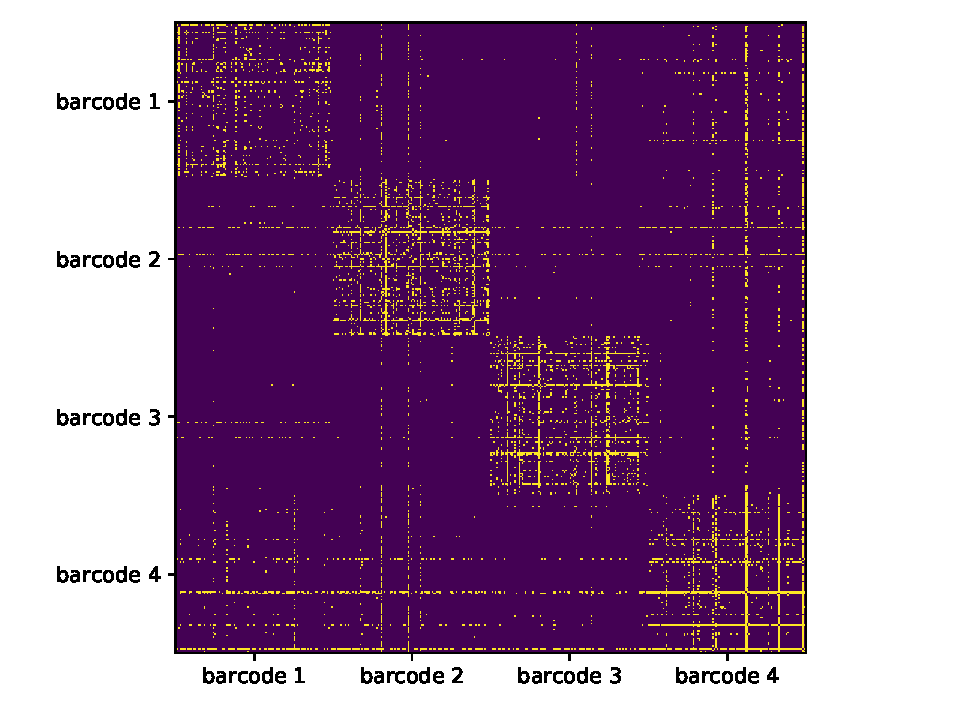
\includegraphics[width=13.5cm]{images/2000_knn_50.pdf} }}%
    \qquad
    \subfloat[$k$NN for $k=150$]
    {{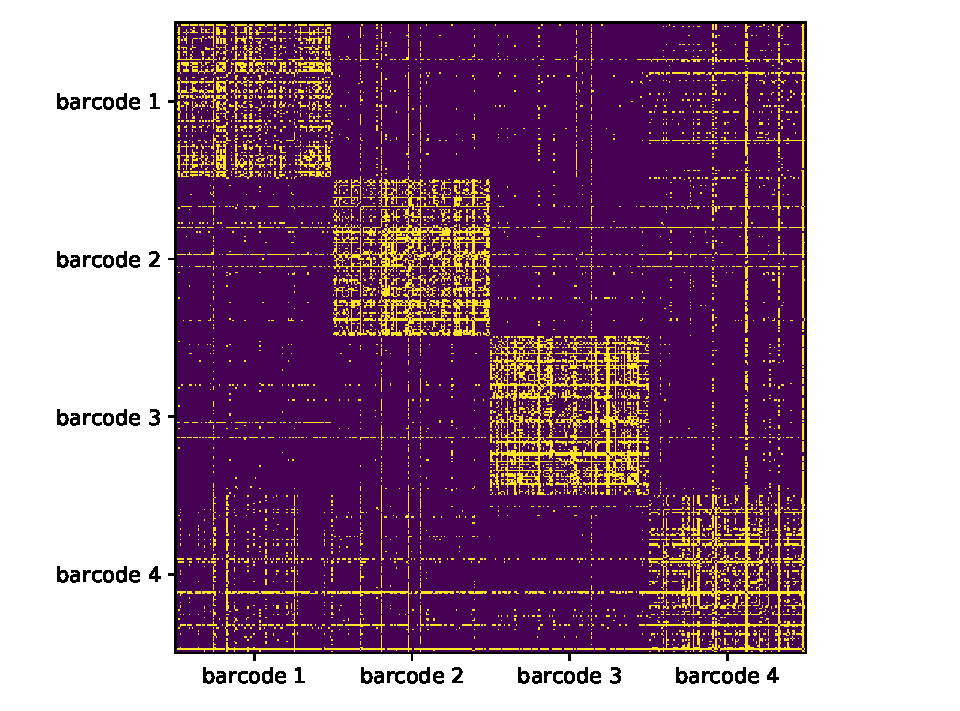
\includegraphics[width=13.5cm]{images/2000_knn_150.pdf} }}%
    \caption[Adjacency matrices of $k$NN graphs]{An example of a LDTW similarity matrix processed into $k$NN adjacency matrix for two choices of $k$. The yellow colour marks the presence of edges. We see that the local neighbourhoods of barcode classes are better outlined for $k=150$ than for $k=50$. The barcode samples are balanced to $500$ samples out of each class for the sake of this visualization.}%
    \label{fig:knn_graphs}%
\end{figure}


\begin{figure}
    \centering
    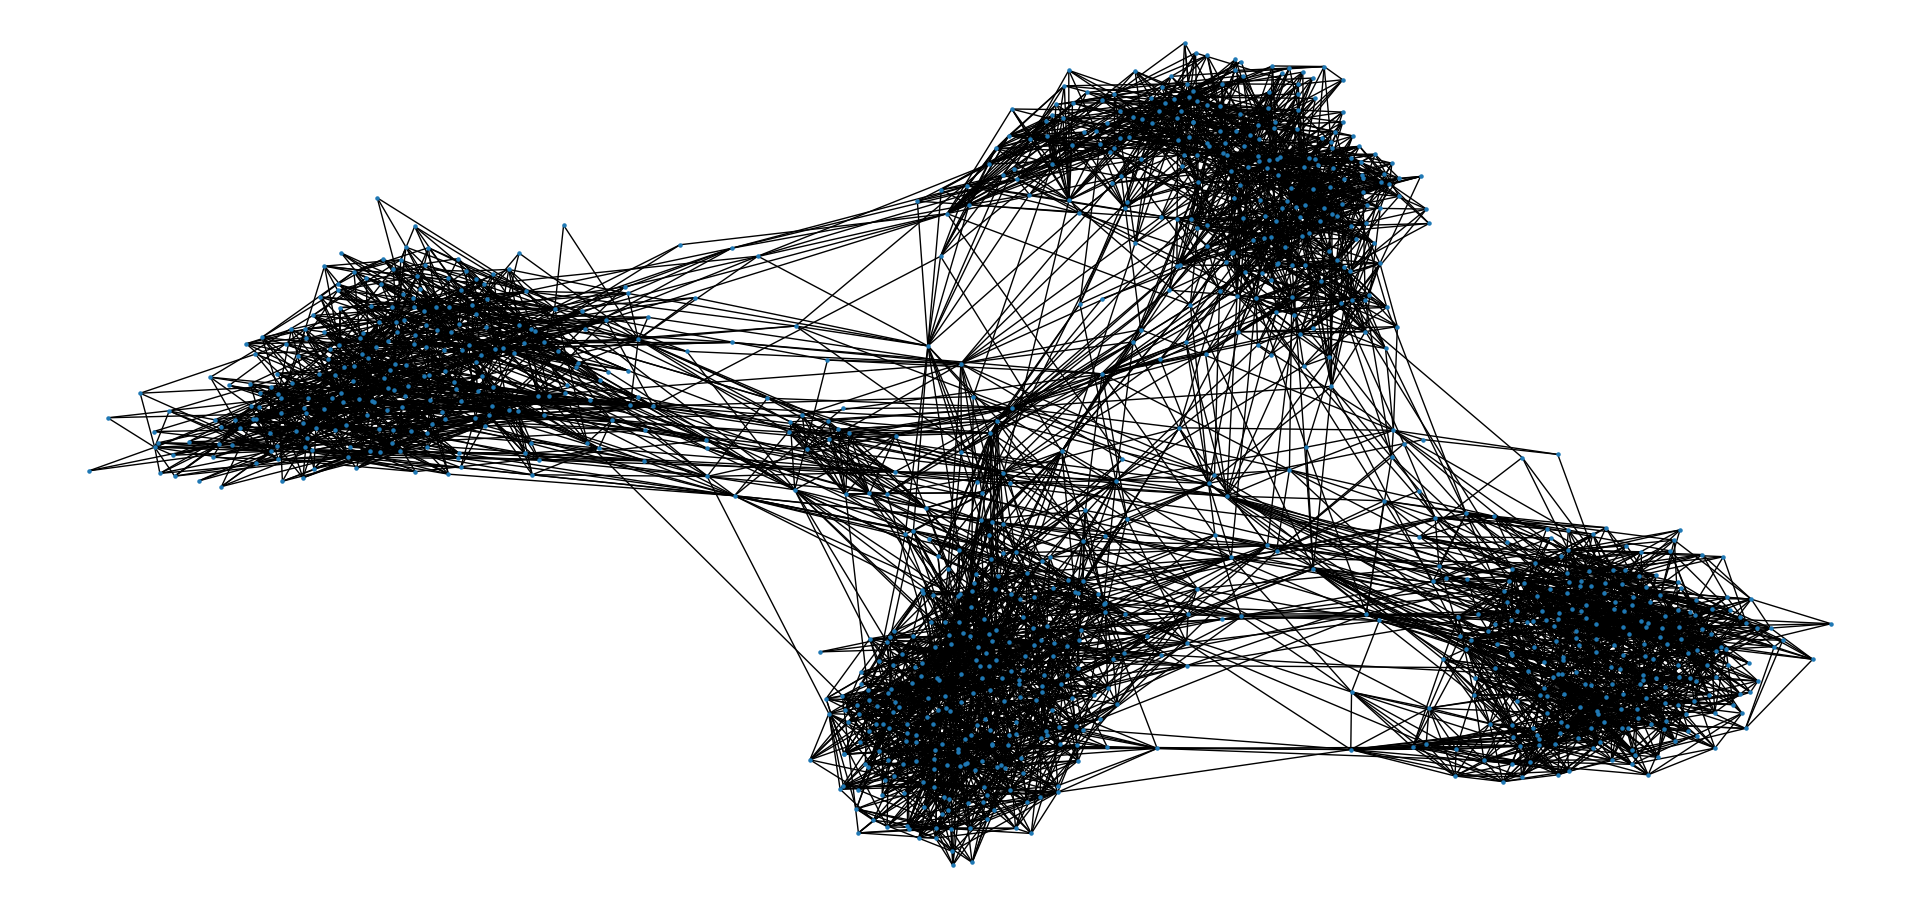
\includegraphics[width=1.0\textwidth]{images/knn_graph_1000.png}
    \caption[$k$NN graph]{A $k$NN graph visualisation for $k=20$ of $1000$ squiggles of barcodes $1-4$ ($250$ squiggles out of each barcode). The visualization was made using the Python module NetworkX \cite{hagberg2005networkx}. The four barcode clusters are clearly identifiable.}
    \label{fig:knn_graph_1000}
\end{figure}

It is indeed a question of great interest how to choose a graph construction method and the corresponding values of the parameters $\sigma, k, \epsilon$ leading to the optimal performance. Let us first address the choice of the graph construction method. Von Luxburg recommends using $k$NN as a first choice to experiment with as it does not appear to be as vulnerable to wrong choices of parameters as the other two methods \cite{von2007tutorial}.

Unfortunately, there is almost no theoretical basis to aid us in the choice the of parameters $\sigma, k, \varepsilon$  \cite{von2007tutorial}. Some theoretical results exist in limit case of $n \to \infty$, such that the $k$NN graph is connected if $k \approx \log(n)$ \cite{von2007tutorial, brito1997connectivity}, but results like these are not very relevant in our scenario. The empirical evidence shows that a 'rule of the thumb' holds for all three of the parameters $\sigma, k, \varepsilon$ - that the parameter must not be too low, neither too high, but somewhere in the middle.

\section{Quality Measures}
In this section we introduce several measures to assess the quality of outputs of our algorithm, both from classification and clustering point of view.

\subsection{Classification Accuracy Evaluation}
\label{sec:classification_metrics}
With the help of \textit{depermutation} we are able to map clusters to barcode classes and subsequently measure the classification accuracy in our experiments. The evaluation is not straightforward since we have multiple classes and will also attempt to detect uncertain label assignments and label them as \textit{no barcode}, which is significantly more tolerable than misclassification. The measures of accuracy that we use in our evaluation are as follows \cite{tharwat2018classification}:

\begin{itemize}
    \item \textbf{Binned reads} - the total number of reads that were assigned a barcode label (i.e. all processed reads without the \textit{no barcode} label, see \cite{Deepbinner})
    \item \textbf{Precision} - or the \textbf{P}ositive \textbf{P}redictive \textbf{V}alue (PPV) is the percentage of binned reads that were labeled correctly
    \item \textbf{Recall} - is the percentage of correctly labeled reads out of all input reads (regardless of being labeled or not)
    \item \textbf{Contingency table} - is a basic classification assessment tool. For a problem of classification into $k$ classes, the contingency table $C$ consists of $k$ rows and $k$ columns. An entry $c_{ij}$ of $C$ is the number of points of predicted class $i$ with the true class $j$. 
    \item \textbf{F-score} - is a classification measure that attempts to unite the notions of precision and recall into a single score. The score is defined as a harmonic mean of precision and recall: $\text{F-score} = \frac{2}{\text{precision}^{-1} + \text{recall}^{-1}}$. Its range spans across the interval $[0, 1]$, where higher values signify better performance. There are several ways of adapting the F-score to deal with multiple-class classification, we will use the one that does not distinguish the particular classes, but measures the accuracy as a whole. When the importance of recall and precision differs, a weighted version $F_{\beta}$ was introduced to account for the imbalance. The original version in terms of the weighted one is referred to as $F_1$ \cite{tharwat2018classification}.
\end{itemize}

\subsection{Clustering Accuracy Evaluation}
Measuring the quality of a clustering is a task more difficult than in the case of classification. In some cases it can even be computationally as hard as the clustering task itself. The methods for clustering output validation can be naturally divided into two categories, namely \textbf{internal} validation and \textbf{external} validation.

In the internal validation the methods have access to the data, the similarity measure, and the predicted labels from the algorithm. In the external validation, on the other hand, the assessment is based purely on the predicted labels and the ground truth labels.

\subsubsection{Silhouette score}
Silhouette score by Peter Rousseeuw \cite{rousseeuw1987silhouettes} is an internal validation method that assesses the quality of a clustering by constructing so called \textit{silhouettes}.
For the construction of silhouettes we will use two additional measures. Without loss on generality, we can again assume that our dataset is the set of the first $n$ natural numbers - $\{ 1, 2, ..., n\}$ and the $k$ ($k > 1$) clusters (an already existing output from some clustering algorithm) are denoted by $\mathcal{C}_1, \mathcal{C}_2, ..., \mathcal{C}_k$, and as was stated before, $\mathcal{C}(i)$ is the cluster that $i$ is a member of. Firstly, let

\begin{equation}
    a(i) = \frac{1}{n} \sum_{j \in \mathcal{C}(i),~ j \neq i} d(i, j),
\end{equation}

so $a(i)$ is the average similarity between $i$ and other points in the cluster of $i$. Now, let $d(i, \mathcal{C}_j)$ be the maximal similarity of point $i$ to any point of cluster $\mathcal{C}_j$. Then, let

\begin{equation}
    b(i) = \max_{\mathcal{C}_j ~\neq~ \mathcal{C}(i)} d(i, \mathcal{C}_j),
\end{equation}

where the $\min$ operator iterates over all clusters other than $\mathcal{C}(i)$. Intuitively, $b(i)$ is the distance to the second closest cluster of data point $i$. We can now  define a silhouette $s(i)$ for a data point $i$ as

\begin{equation}
    s(i) = \frac{a(i) - b(i)}{\max \{ a(i), b(i) \} }.
\end{equation}

Clearly, $s(i)$ takes on values from the range $[-1, 1]$. The case where $s(i) \approx 1$ occurs is the one where the similarities within the assigned cluster are much larger than those to the second closest, and so the clustering is close to perfect. When $s(i) \approx 0$, the situation is that $i$ lies somewhere in between the assigned and second closest cluster, so the assignment is ambiguous. Finally, $s(i) \approx -1$ signalizes that the second closest cluster would be much better cluster for $i$ to be a member of, so the measured assignment is poor.

Silhouette scores require computation of similarities between all pairs of data points, hence becomes infeasible to use with large datasets. However, the computation does not require the ground truth labels that may be sometimes unavailable and can also be used to determine the optimal number of clusters \cite{silhouette1987}. To aggregate the silhouette scores of all data points into one score value, we will use the mean value across all $s(i)$ and denote it as \textbf{S}.

It is also important to note that the Silhouette scores assume that the similarities are on a \textit{ratio scale} - that means similarity of $200$ can be thought of as a double of the similarity of $100$. We we will assume that this does hold for our LDTW similarity.

\subsubsection{Rand index}
Rand Index developed by William M. Rand in $1971$ \cite{randIndex} is an intuitive, external validation method. It is based on observing the frequency of agreements between the predicted and ground truth labels. In more detail, if we were to draw a pair $p_i, p_j$ from the predicted labels and its corresponding pair $t_i, t_j$ from the ground truth labels, exactly one of the four cases occurs:

\begin{enumerate}
    \item $p_i = p_j$ and $t_i = t_j$ - true positive (TP)
    \item $p_i \neq p_j$ and $t_i \neq t_j$ - true negative (TN)
    \item $p_i = p_j$ and $t_i \neq t_j$ - false positive (FP)
    \item $p_i \neq p_j$ and $t_i = t_j$ - false negative (FN)
\end{enumerate}

The Rand Index - $\textbf{RI}$ - of the clustering is then defined as

\begin{equation}
\textbf{RI} = \frac{TP+TN}{TP+TN+FP+FN} = \frac{TP+TN}{\binom{n}{2}}
\end{equation}

The last equality holds because $TP+TN+FP+FN$ is essentially the number of all pairs of the $n$ items, which is trivially $\binom{n}{2}$. As we can observe, $\textbf{RI}$ only takes on values from the range $[0, 1]$. Again, we look at its extremes for interpretation. Intuitively, the value of $1$ signalizes perfect clustering since all drawn pairs of data agree on equality or inequality in predicted labels and ground truth labels and vice versa for $0$, which signalizes that exactly the opposite to the clustering goal has been reached. Values near $0.5$ are those that random cluster assignment would yield. This may lead us to an interpretation that $\textbf{RI}$ is the probability of a data pair agreeing in the prediction and ground truth labelings. However, this is only partially true: it does hold exclusively when we have clusters of equal sizes, which is many times not the case \cite{hubert1985comparing}. For that matter, Hubert et al. \cite{hubert1985comparing} devised an \textit{\textbf{A}djusted \textbf{R}and \textbf{I}ndex} ($\textbf{ARI}$), that corrects the original Rand Index for chance:

\begin{equation}
\textbf{ARI} = \frac{
\textbf{RI} - \text{expected}~ \textbf{RI}
}{
 \text{maximum}~  \textbf{RI} - \text{expected}~ \textbf{RI}
}
\end{equation}

In this way, the $\textbf{ARI}$ represents the probability that a pair of data points has concordant (both TP or TN) label pairs. The span of the $\textbf{ARI}$ is $[-1, 1]$ as can easily be seen. The interpretation of its values is similar to the original $\textbf{RI}$. Both $\textbf{RI}$ and $\textbf{ARI}$ are symmetrical (in the sense that it does not matter which set labels is predicted and which is ground truth).

We must need to note, however, that \textbf{ARI} is only partially related to classification precision. High precision implies high \textbf{ARI}, but when \textbf{ARI} is being low, the precision can only be low.

\subsection{Experiment: Selection of Method for Graph Construction}
\label{sec:graph_construction_experiment}
In this Section, we examine the variety of graph constructions and the suitability of spectral clustering for our problem in a simplified setting. We will work with our two datasets Base and Deepbinner introduced in Chapter \ref{kap:data} (barcoded by Native Barcoding Kit), but will only use barcodes $1-4$. In the Deepbinner dataset, the distribution of squiggles labeled by these barcodes is more or less balanced, with a slight domination of barcode $2$, as opposed to the Base dataset where the squiggles are non-trivially imbalanced and only a handful of squiggles is assigned to barcode $4$. For this experiment, we choose the sample size $N=2000$.

From these squiggles, we will extract prefix and suffix windows by first trimming the blank prefixes/suffixes by our trimming heuristic (also described in Chapter \ref{kap:data}). The extracted windows will be of length $1000$. We then compute the pairwise similarities using the C++ implementation of our \textsc{LDTW} algorithm. Eventually, we end up with two matrices $\textbf{P}$ and $\textbf{S}$ (for \textbf{p}refix and \textbf{s}uffix windows, respectively) of dimension $N \times N$.

There is a large space of possibilities in aggregating the similarity scores to achieve the best result. We can divide these aggregation methods into $2$ categories:

\begin{enumerate}
    \item Merge the score matrices into a single one (e.g. use $\textbf{P}+\textbf{S}$) which is then used for clustering.
    \item Perform the clustering on each score matrix independently and subsequently use the labels from both clusterings to produce a final set of labels.
\end{enumerate}

In the first case, we could be able obtain a more robust and confident similarity matrix, while the second case offers us a natural way of identification of ambiguous label assignments: reads with disagreeing labels on the ends could be labeled as \textit{no barcode} (or 'chimeric', see \cite{Deepbinner}). However, since the goal of this phase is to roughly identify the clusters for further processing and we will address the topic of ambiguous labels assignments later in this work, we will, for simplicity, prefer the additional confidence given from the sum of similarities. Additionally, we will also keep a track of the performance based exclusively on the single front barcodes.

The sampled matrices will serve as an input to spectral clustering, an implementation of which can be found in \texttt{scikit-learn} library \cite{scikit-learn} for the Python language, which we will use. As for the graph construction methods, we employ the notion of a Gaussian similarity function and the $k$NN graph. Even though the Gaussian similarity function is originally defined for real-valued vectors, we can convert our LDTW similarities to distances and then scale them in the Gaussian fashion. We convert similarities to distances by a simple transformation that consists of inverting the signs of the similarity matrix and then shifting the values so that they are non-negative. The Gaussian similarity of squiggles $s_i, s_j$ will then be computed as $G(s_i, s_j) = \exp \Big( \frac{d_{ij}}{2\sigma^2} \Big)$, where $d_{ij}$ is the distance corresponding to similarity $s_{ij}$.

We examine the effects of a range of choices for $\sigma$ (a parameter for the Gaussian similarity) and $k$ (a parameter for the $k$NN). In particular, we examine $k \in \{50, 100, 150, 200, 250\}$ and $\sigma$ will always be set to the mean similarity to the $k$-th nearest neighbor.

We perform $10$ epochs (i.e. independent runs) on each dataset. In each epoch we calculate the $\textbf{ARI}$, the mean silhouette score $\textbf{S}$, and recall of the spectral clustering for the particular variant of graph construction. The silhouette score $\textbf{S}$ is calculated on the original similarity matrix without the adjustments made by individual methods (though the similarities were converted to distances prior to the calculation, since the \texttt{scikit-learn} implementation of silhouette score only supports distances). Finally,  we report the average of these metrics across the $10$ epochs for each variant of graph construction.


\begin{table}[!htbp]
\centering
\begin{tabular}{lccc|ccc}
\toprule
 &  \multicolumn{3}{c}{Base dataset} & \multicolumn{3}{c}{Deepbinner dataset}\\
\midrule
Graph construction method  & ARI   & Silhouette    & Recall (\%) & ARI  & Silhouette    & Recall(\%) \\
\textbf{P} knn50 & 0.73 & 0.27 & \textbf{87.48} & 0.80 & 0.19 & \textbf{91.22} \\
\textbf{P} knn100 & 0.73 & 0.27 & 87.46 & 0.80 & 0.20 & 91.09 \\
\textbf{P} knn150 & 0.73 & 0.27 & 87.42 & 0.79 & 0.21 & 90.75 \\
\textbf{P} knn200 & 0.73 & 0.27 & 87.38 & 0.79 & 0.21 & 90.48\\
\textbf{P} knn250 & 0.73 & 0.27 & 87.34 & 0.78 & 0.21 & 89.99\\
\textbf{P} gauss50  & 0.44 & 0.20 & 67.52 & 0.55 & 0.28 & 69.85 \\
\textbf{P} gauss100 & 0.44 & 0.20 & 67.52 & 0.55 & 0.28 & 69.85 \\
\textbf{P} gauss150 & 0.44 & 0.20 & 67.52 & 0.55 & 0.28 & 69.85 \\
\textbf{P} gauss200 & 0.44 & 0.20 & 67.52 & 0.55 & 0.28 & 69.85\\
\textbf{P} gauss250 & 0.44 & 0.20 & 67.52 & 0.55 & 0.28 & 69.85\\
\hline
\textbf{P+S} knn50 & 0.75 & 0.28 & 87.60 & 0.87 & 0.18 & 94.54\\
\textbf{P+S} knn100 & 0.75 & 0.27 & 87.79 & 0.87 & 0.18 & \textbf{94.57}\\
\textbf{P+S} knn150 & 0.75 & 0.26 & \textbf{87.88} & 0.87 & 0.18 & 94.33\\
\textbf{P+S} knn200 & 0.75 & 0.26 & 87.87 & 0.87 & 0.19 & 94.05\\
\textbf{P+S} knn250 & 0.75 & 0.26 & 87.78 & 0.86 & 0.19 & 93.68\\
\textbf{P+S} gauss50  & 0.55 & 0.24 & 74.76 & 0.63 & 0.22 & 81.17\\
\textbf{P+S} gauss100 & 0.55 & 0.24 & 74.76 & 0.63 & 0.22 & 81.18\\
\textbf{P+S} gauss150 & 0.55 & 0.24 & 74.76 & 0.63 & 0.22 & 81.19\\
\textbf{P+S} gauss200 & 0.55 & 0.24 & 74.76 & 0.63 & 0.22 & 81.23\\
\textbf{P+S} gauss250 & 0.55 & 0.24 & 74.76 & 0.63 & 0.22 & 81.24\\
\bottomrule
\end{tabular}
\caption[The effects of graph construction.]{The effects of graph construction. \textbf{P} stands for prefix barcode only, \textbf{P+S} for the summation of scores from both prefix and suffix.}
\label{tab:matrix_preprocess}
\end{table}

The results are summarized in Table \ref{tab:matrix_preprocess}. Apparently, the Gaussian similarity graph performs significantly worse in overall than than the $k$NN graph, which could be due to infeasible choices of $k$ for their setting of $\sigma$ parameter. The performance seems to be best for $k \in \{50, 100, 150\}$. These results may be biased by only considering a limited variety of data distributions, however, it gives us a notion of how to set the correct parameters for such an experiment. To better outline the local neighbourhoods of graphs with a larger number of barcodes used, the experimenter should choose a lower value of $k$.


\section{Implementation Details}
The bulk of our experiments was written in the Python language for its simplicity and availability of many various libraries for scientific computing. The limiting factor is its low performance when it comes to processing large amounts of data. 

\begin{figure}
    \centering
    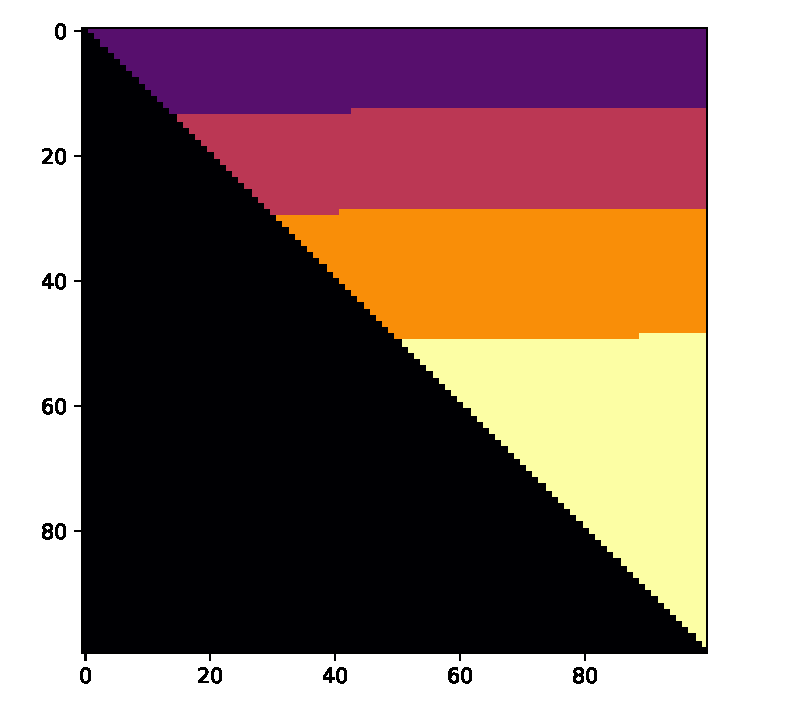
\includegraphics[scale=0.8]{images/equiload_100.pdf}
  \caption[LDTW matrix parallelization ]{A division of a $100 \times 100$ upper triangular matrix into $4$ parts of equal sizes. Each color represents the part assigned to a particular thread, the black part is not processed.}
  \label{fig:equiload_100}
\end{figure}

To address this issue, we have implemented the LDTW algorithm in C++ and used the \texttt{pybind11} \cite{pybind11} library that allows calling subroutines from compiled C++ binaries in Python programs. While offering a minimalistic, but easy-to-use interface, \texttt{pybind11} also provides an automatic conversion of elementary data types between the two languages, which comes in handy when passing nested structures.

\subsection{LDTW Matrix Computation}
In various parts of our experiments, a need for computing a large number of LDTW alignments arose, mostly between all pairs of some set of squiggles. As computing alignments in Python is very slow, we implemented this feature in C++ as a fairly general and flexible function and subsequently linked it to Python as was needed.

We may further observe that computing alignments between all pairs of a set of sequences is an example of an \textit{embarrassignly parallel} \cite{multiprocessor} problem, i.e. a problem to which parallel computing can be applied without much labor, because the threads only require little or no communication flowing between them, which is exactly our case.

To achieve the highest possible utilization of resources, we implemented LDTW matrix computation so that it can be computed in parallel with any number of threads specified in the value of the $N_{\text{threads}}$ variable. This is done by partitioning the matrix into $N_{\text{threads}}$ parts of equal length, each of which will be processed by a single thread. In cases where we only need to compute a half of the LDTW matrix (e. g. due to symmetricity), it is trivially possible use the same approach, as can be seen in Fig. \ref{fig:equiload_100}.


\section{The Clustering Phase}
Our goal is to perform clustering of a potentially very large pool of squiggles (in the order of millions), hence we cannot operate in time complexity asymptotically much greater than linear. Even the constant factor might be critical with dataset being this large.

The problem we attempt to solve is a very specific case of data stream clustering. Its main distinctive features include:

\begin{itemize}
    \item Since we work with time series, we are limited to perceiving the shape of the dataset by observing similarities in pairs by alignments, extracting features is difficult.
    \item Similarity computation between a pair of data is rather costly, we cannot afford to compute it between all pairs of data points.
    \item The stream if always finite.
    \item We have no assumption about the distribution of data among clusters, so the clusters may be arbitrarily imbalanced.
    \item Clusters can theoretically differ in density.
    \item The number of clusters is known prior to clustering and does not change in time.
    \item The whole dataset will probably not fit in into a main memory and so needs to be processed by chunks. However, the dataset of extracted prefixes and suffixes might fit (see \cite{Deepbinner}).
\end{itemize}

We therefore adapt certain ideas from the data stream clustering field and present our approach to the problem in the following sections.

\subsection{Clustering of Data Streams}
In the last few decades we have been witnesses of an increase in volume of practically handled data by several orders of magnitude. This emphasized the drawbacks of many clustering algorithms that are often incapable of processing large amounts of data and efficiently adapting to new coming data points \cite{silva2013data}. The model of a data stream is essentially an enormously large sequence of data, potentially unbounded, therefore impossible to fit in main memory. The clustering models that process this kind of data are therefore not allowed to grow in size at any rate with the new coming data \cite{silva2013data}. 

The article \textit{Data Stream Clustering: A Survey}  by Jonathan A. Silva et al. \cite{silva2013data} is a complex summary of methods developed for clustering of data streams along with their characteristic features, parameters they need, time and memory complexities, etc.

\begin{figure}[]
    \centering
    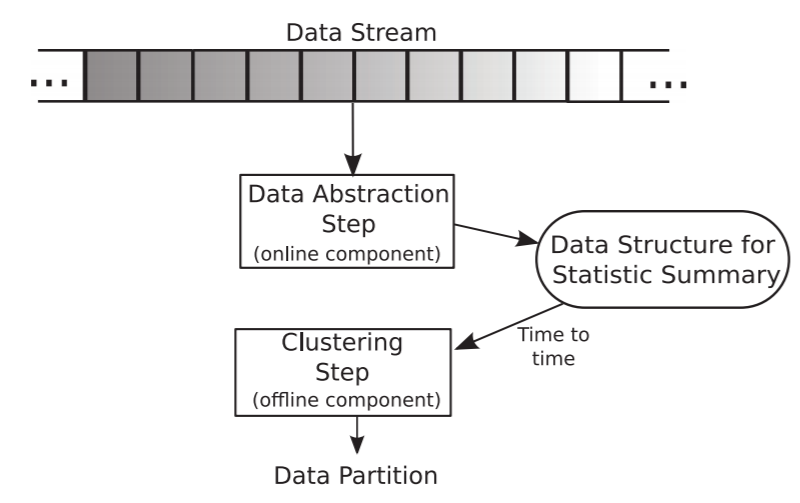
\includegraphics[width=15.5cm]{images/stream_clustering_scheme.png}
    \caption[Clustering of data streams scheme]{A high level abstraction of how most data stream clustering algorithms work \cite{silva2013data}.}
    \label{fig:stream_clustering}
\end{figure}

Most data stream clustering algorithms consist of two types of components. The first the \textit{online} component which performs the \textit{data abstraction step} - i.e. managing the new coming data, updating the model, deciding what data to keep and what to discard, etc. The \textit{online} component performs the \textit{clustering} step, which is usually an old-fashioned non-stream clustering algorithm \cite{silva2013data}. This scheme is sketched in Fig. \ref{fig:stream_clustering}.

\subsection{Experiment: DBSCAN}
\textbf{D}ensity-\textbf{b}ased \textbf{s}patial \textbf{c}lustering of \textbf{a}pplications with \textbf{n}oise or its acronym DBSCAN \cite{schubert2017dbscan}, is a clustering algorithm. As is reflected in its name, the decisive factor in the clustering process is the density of the data. Our idea was to divide the squiggle dataset into chunks of reasonable sizes, so that each of them could be subsequently independently clustered by DBSCAN and the clusters corresponding to individual barcode classes would be unified in the final step.

DBSCAN works by iterating through data points constructing a so-called \textit{core points}, which are data points that have at least \texttt{minPts} points in their $\varepsilon$-neighbourhood. All points that lie within the $\varepsilon$-neighbourhood of a core point are part of the same cluster. If any of these points is a core point, then its $\varepsilon$-neighbourhood is also included in the cluster in a transitive fashion \cite{schubert2017dbscan}. When a point is unreachable from any existing cluster, it is labeled as \textit{noise} \cite{schubert2017dbscan}. Therefore, DBSCAN does not require the number of clusters in the input, the 'optimal' number is inferred from the data.

We performed a number of experiments with our LDTW similarity function, with various values of parameters for $\varepsilon$ and \texttt{minPts}, but could not find a configuration that would achieve other than poor results. As the performance of DBSCAN is heavily influenced by the $\varepsilon$ parameter, we carefully searched for the right value that would enable DBSCAN to identify the clusters, but even in a perfectly balanced sample it only lead to unsatisfactory results - the higher values lead to labeling most (or all) of the reads as the same class, the lower values caused that most of the reads were labeled as noise and we could not find a balance between these extremes.

This could be explained by the fact that the cluster are topologically connected, as is reflected in the MDS visualisation in Figures \ref{fig:2000_MDS_2D} and \ref{fig:2000_MDS_3D}. Low values of $\varepsilon$ isolate the squiggles in their own clusters when $\varepsilon$ becomes large enough to make connections, the whole sample becomes densely connected.

\subsection{Aligning to Representatives}
In Section \ref{sec:suitable_clustering_algorithms}, we provided a motivation for the use of spectral clustering for moderate dataset sizes and in Section \ref{sec:graph_construction_experiment} we tested it with our LDTW algorithm as a similarity metric. This offers us an idea of adapting the spectral clustering to a setting with large datasets, which we may think of as an online version of the problem.

There has been many efforts of adjusting SC algorithms to a scenario when data come in a stream fashion. These algorithms mostly fall into one of the two main categories \cite{kong2011fast}: 

\begin{itemize}
    \item \textbf{Eigenvalue update approximation:} algorithms that attempt simulating an update of the eigenvalue system in an efficient way to account for the re-computation of the whole clustering as data points come.
    \item \textbf{Clustering according to representatives:} picking a set of data points - representatives - from each cluster that would serve as a guide to assigning cluster labels to the additional data points.
\end{itemize}

We focus on the latter method because the notion of a set of representative squiggles comes fairly naturally. Would we be able to pick reliable representatives, we could efficiently and accurately cluster the rest of the squiggles by aligning them to the representatives and inferring the cluster label from the alignment scores. To be able to pick the representatives, we may first sample a small pool of squiggles, compute the all pairs LDTW scores, use them to cluster the squiggles by the classical spectral clustering, and finally choose the representatives in a suitable way (see Algorithm below).

\begin{algorithm}[H]
\floatname{algorithm}{Algorithm}
\renewcommand{\thealgorithm}{}
\caption{Clustering squiggles by aligning to representatives}
\label{protocol1}
\begin{algorithmic}[1]
\STATE Sample a small set of squiggles $A = \{ s_1, ..., s_n \}$
\STATE Compute a LDTW similarity matrix $S_{n \times n}$ of all pairs in $A$
\STATE Obtain labels for the squiggles in $A$ based on $S$ using spectral clustering
\STATE For each barcode, select $r$ representatives from $A$ based on $S$
\STATE Align the rest of the squiggles to the representatives and assign them to a cluster on the basis of the similarity scores or conclude that the assignment is ambiguous
\end{algorithmic}
\end{algorithm}

The actual choice of representatives in step $5$ is an important subproblem on its own and we will examine it more closely in the next section.

Of course, the more barcodes we use in the sequencing the bigger the initial matrix must be in order to capture a reasonable amount of squiggles from each barcode class in the initial step. The problematic factor might be the class imbalancedness by the cause of which we might need to sample a much bigger matrix in order to obtain a sufficient number of squiggles from each barcode class.

Therefore in this algorithm, the time complexity  and overall performance grows with the number of barcodes used. Our goal is to design an algorithm that could cluster the squiggles sufficiently well and, in the ideal case, independently of the number of barcodes used. We must, however, keep in mind that since our method is unsupervised, that our algorithm can only be as good as the quality of the sequenced squiggles.

\subsection{Selection of Representatives}
When devising the criteria for the selection of representatives, we face a large space of possibilities of combining the LDTW scores in a way that would yield the most distinctive and simultaneously robust representatives sets for each cluster. In this section, we assume that we have already obtained the LDTW scores for the squiggles $s_1, ..., s_m$ and (in any sensible way) the corresponding predicted labels $\ell_1, ..., \ell_m$. We must, however, also keep in mind that the labeling might not be completely reliable (see Tab. \ref{tab:matrix_preprocess}).

We will use a notion of a \textit{\textbf{s}plit \textbf{r}atio \textbf{c}oefficient} - $\textbf{SRC}$ as a function of a data point $i$ to measure the representativeness of the particular data point. Therefore, the motivation behind $\textbf{SRC}(i)$ is to measure how well a particular squiggle $i$ discriminates in the scope of the sample. Let $i_{j1}, i_{j2}, ..., i_{j |\mathcal{C}(j)|}$ be the indices of the squiggles of cluster $j$ sorted in descending order by the their $\textbf{SRC}$ value. The set of the representatives $R_j$ for barcode class $j$ then consists of the first $N_{\text{repr}}$ squiggles by this ordering:

\begin{equation}
    R_j = \{ i_{j1}, i_{j2}, ..., i_{jN_{\text{repr}}} \} .
\end{equation}

For the computation of $\textbf{SRC}$, we devised the following methods:

\subsubsection{Random Selection}
The simplest of the methods is to pick the representatives uniformly at random under the hypothesis that constraining the selection would introduce a bias that would show negatively in the clustering phase. The $\textbf{SRC}_{\text{random}}(i)$ is therefore a randomly generated number.

\subsubsection{Mean Scores Ratio}
This greedy selection takes into the consideration the ratio of mean score value to squiggles within its own class to the mean score value to other classes:

\begin{equation}
    \textbf{SRC}_{\text{means-ratio}}(i) =
        \frac{\text{mean score within its class} }{\text{mean score outside its class} } =
    \frac{
        \frac{1}{|\mathcal{C}(i)| - 1} \sum_{j \in \mathcal{C}(i) ~;~ i \neq j} s_{ij}
    }{
        \frac{1}{m - |\mathcal{C}(i)|} \sum_{j \notin \mathcal{C}(i)} s_{ij}
    }
\end{equation}


\subsubsection{Product Scores Ratio}
To emphasize the importance of maximizing/minimizing the scores inside/outside of its own cluster, we may propose a product of the scores instead of their sum as in the previous method:

\begin{equation}
    \textbf{SRC}_{\text{product-ratio}}(i) =
        \frac{\text{scores product within its class} }{\text{scores product outside its class} } =
    \frac{
        \prod_{j \in \mathcal{C}(i) ~;~ i \neq j} s_{ij}
    }{
        \prod_{j \notin \mathcal{C}(i)} s_{ij}
    }
\end{equation}

To make the scoring scheme numerically stable, we take the logarithm of the whole fraction. This is a standard method of stabilization a computation of long chain products in scientific computing and it relies on the properties of logarithm - due to its monotonicity we know that the rankings will preserve their orderings.

\begin{multline}
    \log \Big( \textbf{SRC}_{\text{product-ratio}}(i) \Big) =
    \log \Bigg(
    \frac{
        \prod_{j \in \mathcal{C}(i) ~;~ i \neq j} s_{ij}
    }{
        \prod_{j \notin \mathcal{C}(i)} s_{ij}
    } \Bigg) =
    \log \Bigg( \prod_{j \in \mathcal{C}(i) ~;~ i \neq j} s_{ij} \Bigg) -
    \log \Bigg( \prod_{j \notin \mathcal{C}(i)} s_{ij} \Bigg) =\\=
    \sum_{j \in \mathcal{C}(i) ~;~ i \neq j} \log(s_{ij}) - 
    \sum_{j \notin \mathcal{C}(i)} \log(s_{ij})
\end{multline}

\subsubsection{Maximum Class Score Ratio}
The final method makes the ratio out of the maximum score from within its own class to the product of maximum scores to other classes to emphasize that the scores to each of the other classes should be low and so to avoid the situation where the ratio is high only due to low scores to a single, dominant cluster.

\begin{equation}
    \textbf{SRC}_{\text{max-class}}(i) =
        \frac{\text{max. score inside its own class} }{\text{product of max. scores from other classes} } =
    \frac{
        \max_{j \in \mathcal{C}(i) ~;~ i \neq j} s_{ij}
    }{
        \prod_{j \neq i} \max_{k \in \mathcal{C}(j)} s_{i, k}
    }
    \label{eq:maxclass}
\end{equation}

As before, we avoid computing the chain products by taking the logarithm of Eq. \ref{eq:maxclass}:

\begin{multline}
    \log \Big( \textbf{SRC}_{\text{max-class}}(i) \Big) = \log \Bigg( \frac{
        \max_{j \in \mathcal{C}(i) ~;~ i \neq j} s_{ij}
    }{
        \prod_{j \neq i} \max_{k \in \mathcal{C}(j)} s_{i, k}
    } \Bigg) = \log \Big(
        \max_{j \in \mathcal{C}(i) ~;~ i \neq j} s_{ij}
    \Big) - \\ - \Bigg(
        \prod_{j \neq i} \max_{k \in \mathcal{C}(j)} s_{i, k}
    \Bigg) = \log \Big(
        \max_{j \in \mathcal{C}(i) ~;~ i \neq j} s_{ij}  \Big) -         \sum_{j \neq i} \log \Big( \max_{k \in \mathcal{C}(j)} s_{i, k} \Big)
\end{multline}

\subsection{Methods of Label Assignment}
The final problem we need to address is the decision making based on alignment scores to representatives. Given a set of LDTW scores to representatives from each barcode class, we need to decide what label to assign to the read, or potentially, conclude that we are unable to assign a label with sufficient certainty.

We devised several methods that might solve this problem. Let us again assume that $s_{ij}$ is the LDTW score of the $i$th read and the $j$th read. We will consider following methods:

\begin{itemize}
    \item \textbf{Maxmean:} The class is inferred by first computing the mean score to representatives from $i-$th class $M_i = \frac{1}{N_{\text{repr}}} \sum_{j \in \mathcal{C}(i)} s_{i, j}$ and then assigning the class according to the maximum value among $M_1, ..., M_{k}$. Additionally, we may introduce a term $\tau$ that will be used to test significance of the assignment - we only assign a class label when the ratio of the second highest $M_{\beta}$ to the highest $M_{\alpha}$ is at least $\tau$.
    \item \textbf{$k$NN:} We can also work in $k$-nearest neighbours fashion - we look at the similarity scores to the $k$ best matches for some small $k$, and assign the class with highest occurrence. In case of a tie we can conclude that the label is ambiguous. Alternatively, we can set $k$ to an even smaller value and only assign a label if all the $k$ nearest neighbours are from the same class. 
    \item \textbf{Spectral clustering:} The final method that we propose to use is again spectral clustering as in the discovery phase. For a squiggle $s$ we will create a set of input squiggles as
    $$ \{ r_{1, 1}, ..., r_{k, N_{\text{repr}}}, s \}$$ where $r_{i, j}$ is the $j-$th representative of the $i-$th class. We will compute its pairwise similarities and run spectral clustering on the generated similarity graph. To depermutate the predicted label, we infer the depermutation $\Phi$ from the predicted labels of $r_{1, 1}, ..., r_{k, N_{\text{repr}}}$ and return $\Phi(s)$. The detection of insignificant labels is a bit more unintuitive in this case. One way to work around this is to use the $k$NN method in the spectral embedding space. Alternatively, we could first detect the ambiguity of assignment by any other method and assign a label using SC if ambiguity is not present.
\end{itemize}

\subsection{Experiment: Grid Search Over Representative Selections and Label Assignment Methods}
In this experiment we will examine the performances of the representative selections and cluster assignment methods we defined earlier. We will perform $10$ epochs of the experiment with the following parameters:

\begin{itemize}
    \item The experiment will be performed independently with the Base dataset and Deepbinner dataset
    \item Sample size for the initial discovery step will be $2000$ squiggles, we will use both prefix and suffix windows, the alignment score from both ends will be added together and a $k$NN graph will be constructed for $k=100$ (as was proved to be reliable earlier)
    \item The number of representatives we set on $N_{\text{repr}} = 25$
    \item $k = 3$ for the $k$NN label assignment method, we will assign the most occurrent label among the $3$ nearest neighbours, for the sake of simplicity in this experiment we will assign a label randomly in case of a tie
    \item We perform a grid search over the representatives selections and cluster assignment methods
    \item In each of the $10$ epochs we will classify $10,000$ reads sampled uniformly at random, using the particular set of selected representatives and assignment method
    \item For label assignment, the scores $s_{ij}$ will be calculated as the sum of prefix and suffix LDTW alignment scores 
\end{itemize}

\subsubsection{Results and discussion}
The results of this experiment are summarized in Tab. \ref{tab:grid_search}. The \textbf{maxclass} representative selection method performs considerably worse in both datasets than other methods. On the other hand, the \textbf{means-ratio} methods appears to be the most robust out of the ones we tested. As for the cluster assignment methods, the \textbf{maxmean} and \textbf{spectral} methods seem to achieve comparable performance that peaks when used jointly with the \textbf{means-ratio} representative selection. As the \textbf{maxmean} method is conceptually much simpler than SC and consequently adds much less complexity to our model, we will use that one for further analyses. The recall achieved in the Deepbinner dataset is actually higher than in the Deepbinner itself (93.33\%, \cite{Deepbinner}), although we must note that our tests were performed on a much smaller testing sets and only using the barcodes $1-4$. In both Base and Deepbinner datasets we achieved recall higher than the one of Albacore ($\approx 85\%$).

\begin{table}[!htbp]
\centering
\begin{tabular}{lcccc}
\toprule
 &  \multicolumn{2}{c}{Base dataset} & \multicolumn{2}{c}{Deepbinner dataset}\\
\midrule
Selection / Assignment & ARI   & Recall (\%) & ARI & Recall (\%) \\
\hline
random / maxmean & 0.75 & 87.58 & 0.84 & 93.31  \\
random / $k$NN & 0.69 & 85.29 & 0.72 & 87.78 \\
random / spectral & 0.74 & 87.29 & 0.82 &  92.45 \\
means-ratio / maxmean & 0.75 & 88.10 & 0.87 & \textbf{94.17}  \\
means-ratio / $k$NN & 0.75 & 88.07 & 0.86 & 93.93 \\
means-ratio / spectral & 0.74 & 87.11 & 0.86 & 94.01 \\
product-ratio / maxmean & 0.75 & 88.67 & 0.31 & 68.63  \\
product-ratio / $k$NN & 0.75 & 88.19 & 0.58 & 82.47 \\
product-ratio / spectral & 0.66 & 81.98 & 0.60 & 78.83 \\
max-class / maxmean & 0.49 & 73.68 & 0.31 & 78.50  \\
max-class / $k$NN & 0.62 & 82.06 & 0.66 & 83.02 \\
max-class / spectral & 0.68 & 83.98 & 0.68 & 85.98 \\
\bottomrule
\end{tabular}
\caption[Representative selection and cluster assignment summary]{This table summarizes the effects of several representative selection and cluster assignment methods. The \textbf{ARI} and \textbf{Recall} values are the average over the $10$ epochs.}
\label{tab:grid_search}
\end{table}

Let us now examine in greater detail the phenomenon of the apparent recall gap between the Base and Deepbinner datasets. The culprit of this sort of a behavior can be hidden behind two facts: the first reason might be the imbalancedness of the barcode classes which forces the spectral clustering to yield more balanced clusters even for the price of a worse solution. The second reason could be the similarity of the barcodes $1$ and $4$ in the signal space and the fact that barcode $1$ becomes very similar to barcode $4$ due to some sequencing artifact.

We computed the all-pairs score matrix made out of $2000$ sampled reads from the Base dataset and ordered its entries according to the their barcode classes, for both ground truth classes and predicted classes. The distribution of the barcodes in this sample was $1040,  334,  564,   62$ for barcodes $1-4$ respectively. The result is displayed in Fig. \ref{fig:true_pred_comparison}, in which we can see that the barcode $4$ seems to be outlined very well even when the matrix is ordered according to the predicted labels.

\begin{figure}[!ht]
    \centering
    \subfloat[True labels ordering]
    {{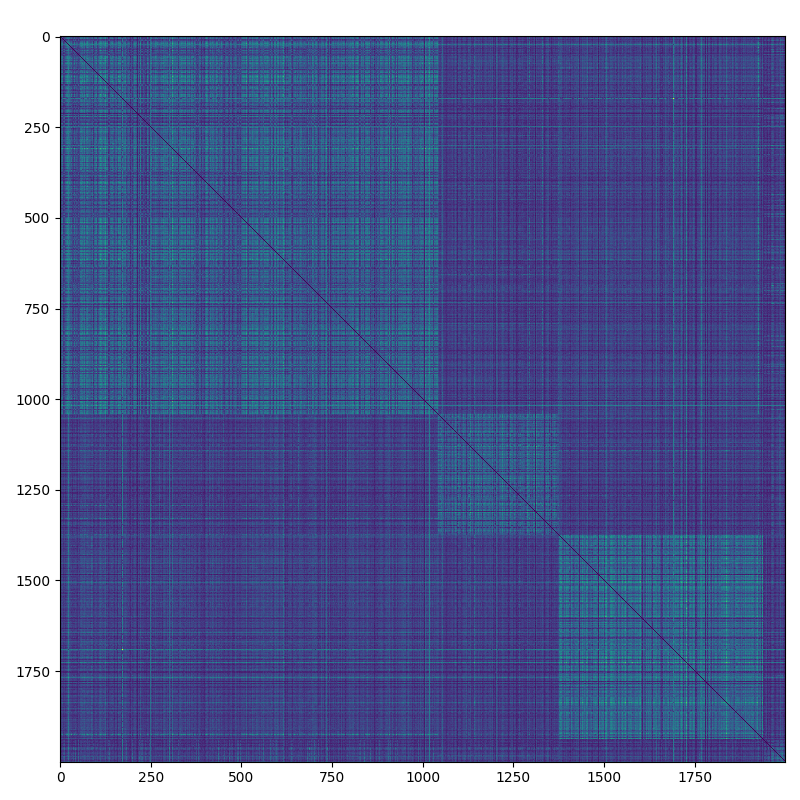
\includegraphics[width=7cm]{images/2000_base_true.png} }}%
    \qquad
    \subfloat[Predicted labels ordering]
    {{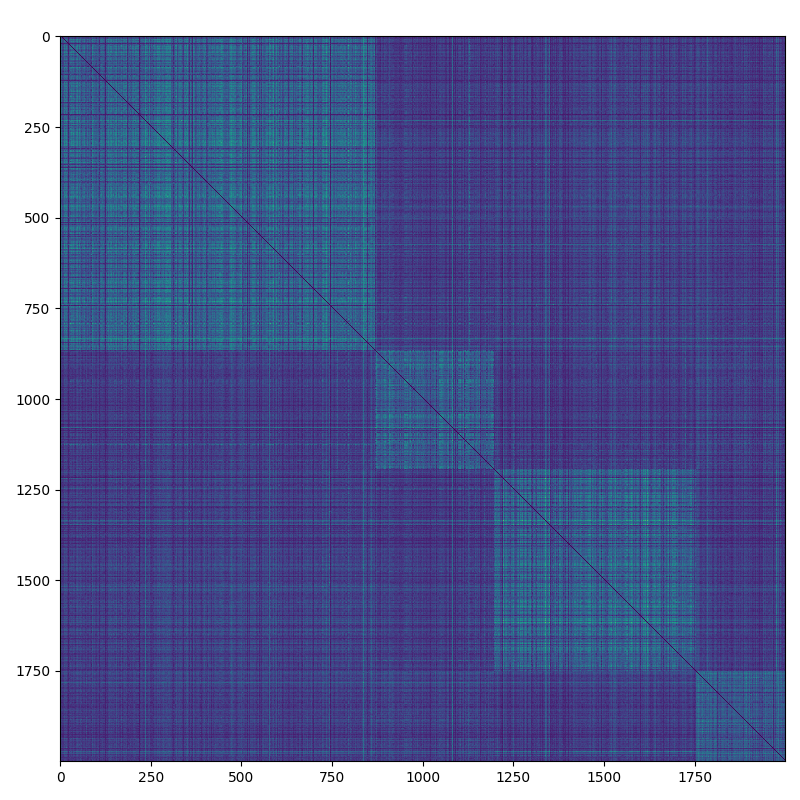
\includegraphics[width=7cm]{images/2000_base_pred.png} }}%
    \caption[Discovery matrices orderings]{Left: The sample of reads ordered according to their ground truth labels. Right: The ordering corresponding to the predicted labels.}%
    \label{fig:true_pred_comparison}
\end{figure}

Let us now compare this to the situation when the barcode classes are balanced. We computed another $N \times N$ ($N=2000$) score matrix of the Base dataset, but with a completely balanced distribution of barcodes $1-4$ (i.e. $500$ barcodes out of each class). Subsequently, we performed the spectral clustering on both of them (also using $k$NN graph for $k=100$) and compared their corresponding contingency matrices in Tab. \ref{tab:two_contingencies}. As we can see, the same phenomenon is present in the balanced sample case, although in a smaller scale. Barcodes $2$ and $3$, on the other hand, seem to be well pronounced with little confusion.
\bigskip

\begin{tabular}{ cc }% top level tables, with 2 columns
\label{tab:two_contingencies}
Contingency table (balanced sample) & Contingency table for (imbalanced sample) \\  
\begin{tabular}{c|c|c|c|c}
& bc 1 & bc 2 & bc 3 & bc 4\\
\hline
bc 1 & \textbf{389} & 0 & 3 & \textbf{108}\\
bc 2 & 1 & 477 & 2 & 20\\
bc 3 & 4 & 2 & 482 & 12\\
bc 4 & 5 & 4 & 9 & 482
\end{tabular} &
\begin{tabular}{c|c|c|c|c}
& bc 1 & bc 2 & bc 3 & bc 4\\
\hline
bc 1 & \textbf{842} & 8 & 5 & \textbf{185} \\
bc 2 & 7 & 318 & 4 & 5\\
bc 3 & 13 & 0 & 547 & 4\\
bc 4 & 7 & 1 & 1 & 53 
\end{tabular}\\
\end{tabular}
\bigskip

We can therefore conclude the presence of at least one phenomenon of the two we mentioned - the mixing of barcode $1$ into barcode $4$. This is  also reflected MDS visualisations in Figures \ref{fig:2000_MDS_2D} and \ref{fig:2000_MDS_3D}.

%\subsection{Experiment 3}
%In this experiment, we will try to enhance the setting of the experiment $1$ with more robustness. Our hypothesis is that independent samples of the training set independently distribute the $15\%$ of errors in the training set. We will therefore be sampling the training set $N_{\text{iter}}$ times and each time calculate the set of labels for the testing set, which was sampled only once at the start. This way we will end up with $N_{\text{iter}}$ sets of labels for the testing set that we need aggregate in some way to a final labeling.

%We will to this by setting $N_{\text{iter}} = 5$ and requiring at least $3$ labels of the same kind to be assigned to a particular read among the iterations. Reads that do not meet this criterium will be considered ambiguous and will be assigned no label ($-1$ in our implementation).

%The results of this experiment were not much different from experiment $1$. The accuracy practically did not improve at all. Upon examining the contingency tables of the testing samples (see Fig. \ref{fig:contingency_matrix1}), we found that as much as $8.7\%$ of the whole testing sample were reads belonging to the barcode class $1$, but were assigned a class $4$. This is simultaneously the vast majority of the errors that were made in each of the independent $N_{\text{iter}} = 5$ runs in this experiment.

%The crucial focus from this point is to find the culprit of this phenomenon and try to find a solution of its elimination.

\subsection{Experiment: The Detection of Ambiguous Labels}
An important factor in barcode assignment is that misclassifying a read and subsequently using it for further analysis is much more severe than disposing of it and not using it at all, because it pollutes the genomic data with spurious samples. Identification of these errors is therefore crucial for the practical usability of the algorithm.

Looking under the cover of our clustering step, we will attempt to design a heuristic that discards those reads whose scores to representatives yield an ambiguous label assignments. As we saw earlier, both \textbf{maxmean} and \textbf{$k$NN} methods offer us natural methods of identification of ambiguous labels. Let us try the \textbf{maxmean}, which seemed to work when we tried a few values of $\tau$ set by hand. We will explore this parameter more thoroughly by performing a search through values $\tau \in \{0, 0.05, 0.1, 0.15,... , 1 \}$ in the clustering phase and for each value we compute the $F$-score defined in section \ref{sec:classification_metrics}. The default $F$-score, however, considers precision and recall as equally important. We, on the other hand, seek to emphasize high precision even for the cost of lower recall. To measure this imbalance, we will employ the $F_{\beta}$ score defined as follows \cite{tharwat2018classification, fbetascore}:

\begin{equation}
F_{\beta} = (1 + \beta^2) \frac{\text{precision} \cdot \text{recall}}{\beta^2 \text{precision}  + \text{recall}},
\end{equation}

where $\beta$ represents the difference of importance between precision and recall. Lower values of $\beta$ emphasize precision, while higher values emphasize recall \cite{fbetascore}. We will experimentally set $\beta = 0.5$. This should give us a more founded idea what value of $\tau$ should be chosen.

We performed an experiment on $10,000$ sampled squiggles from both Base and Deepbinner datasets and performed classification for each value of $\tau$ mentioned earlier, from which we plotted both $F_1$-scores and $F_{\beta}$-scores for $\beta = 0.5$. From the results Fig.\ref{fig:f1_scores}, we see that giving more weight to recall by setting $\beta$ to $0.5$ yields the value of $\tau \approx 0.9$ as optimal.

\begin{figure}[!ht]
    \centering
    \subfloat[$F_1$ Base]    {{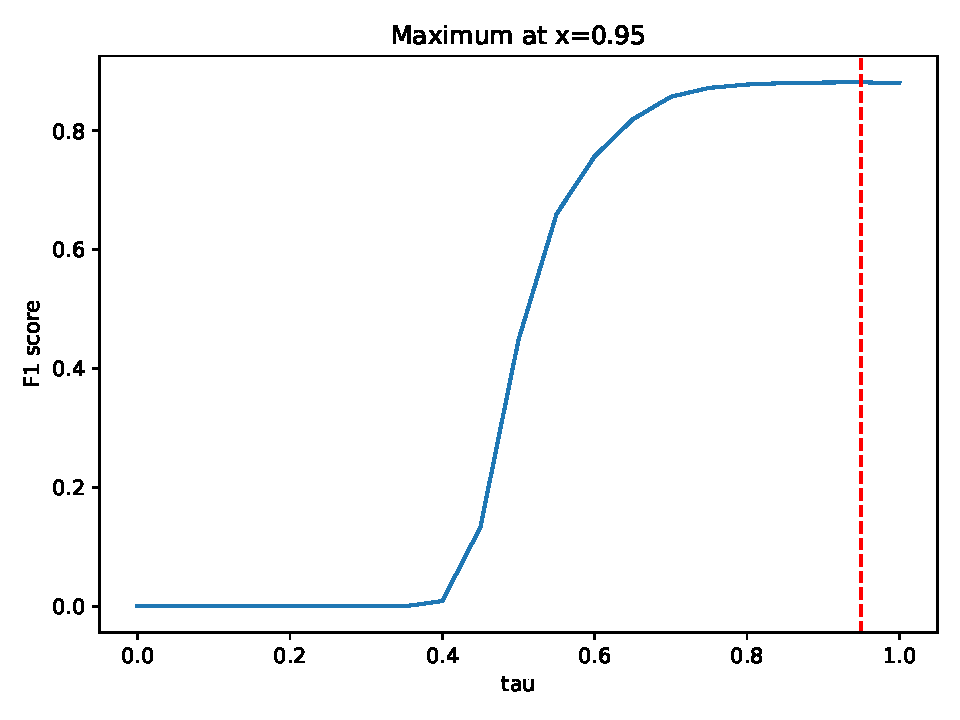
\includegraphics[scale=0.5]{images/f1_mean_maxmean_base.pdf} }}%s
    \subfloat[$F_1$ Deepbinner]
    {{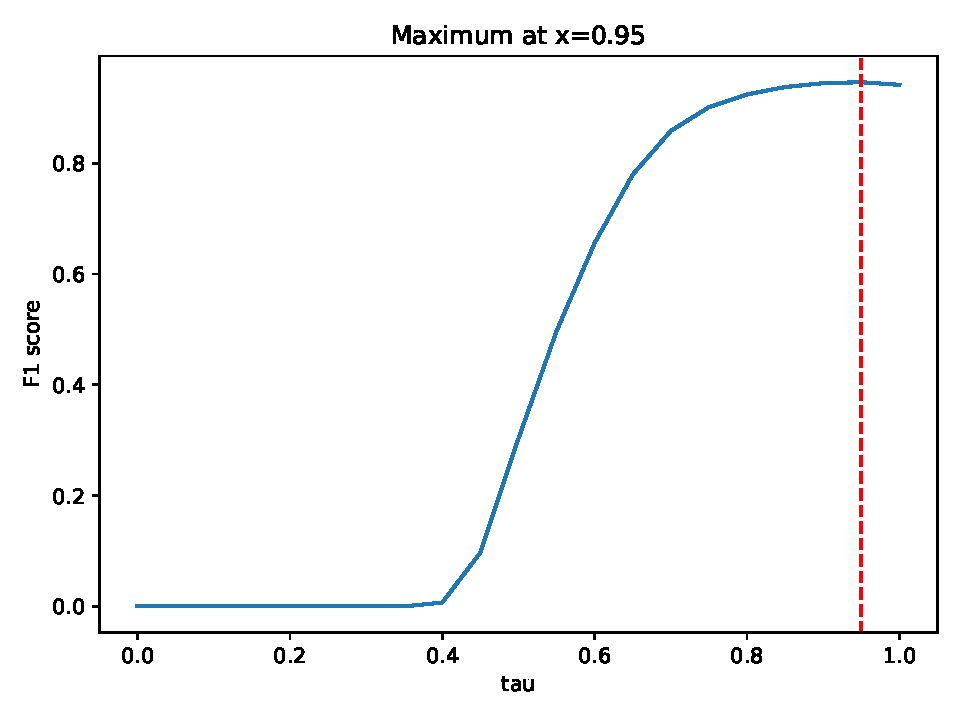
\includegraphics[scale=0.5]{images/f1_mean_maxmean_deepbinner.pdf} }}%
    \qquad
    \subfloat[$F_{\beta}$ Base]
    {{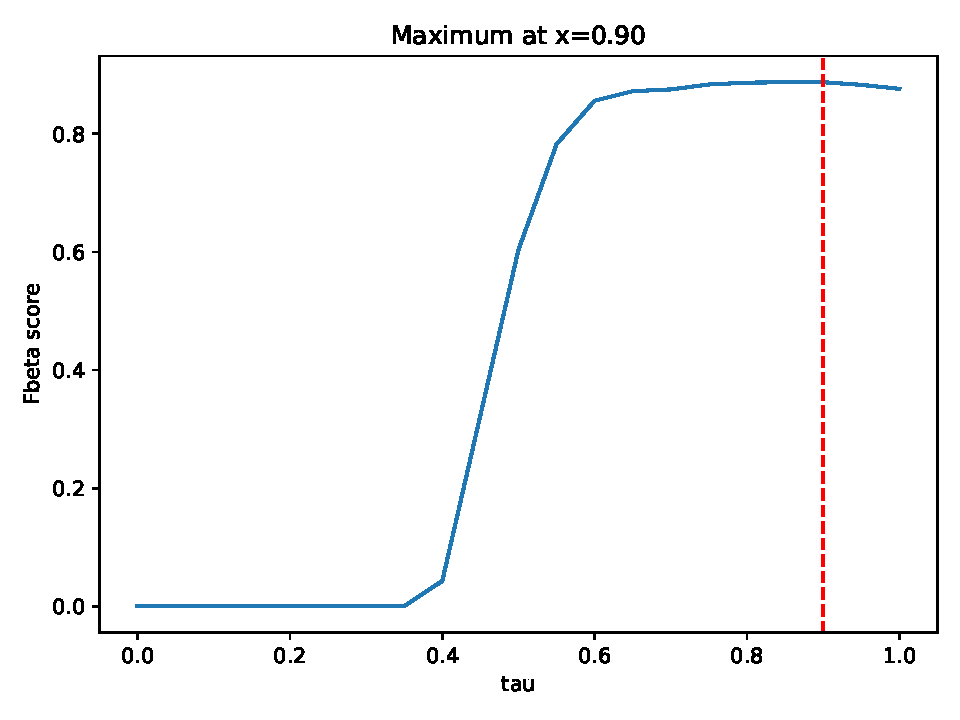
\includegraphics[scale=0.5]{images/fbeta_mean_maxmean_base.pdf} }}%
    \subfloat[$F_{\beta}$ Deepbinner]
    {{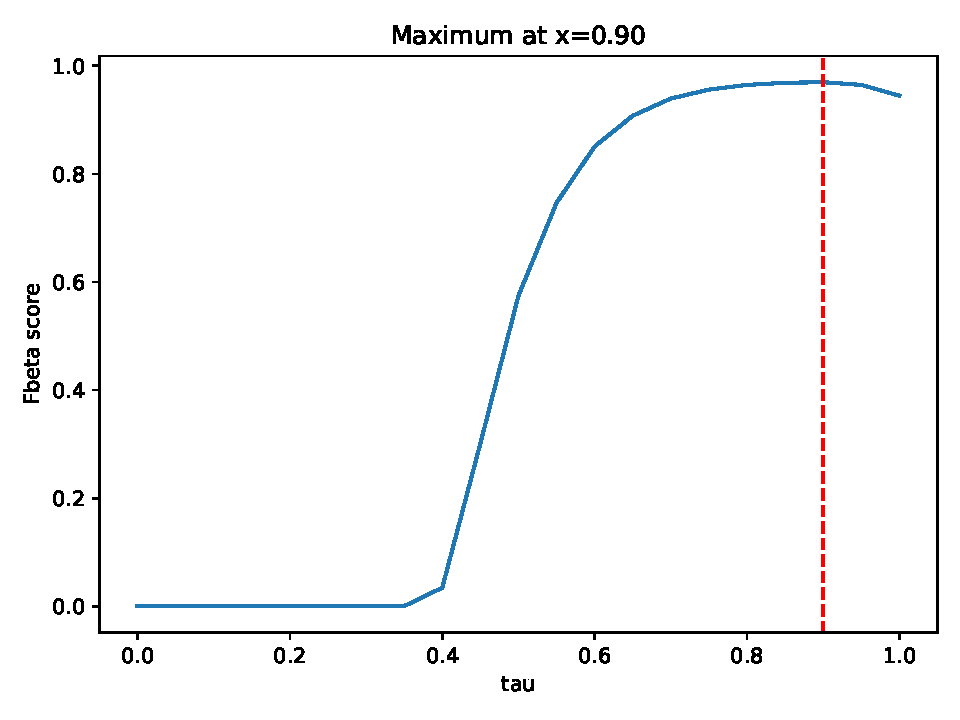
\includegraphics[scale=0.5]{images/fbeta_mean_maxmean_deepbinner.pdf} }}%
    \caption[Scoring scheme construction.]{The dependence of F$1$ score and $F_{\beta}$-score statistic (for $\beta = 0.5$) on the value of $\tau$ for each dataset. The red line marks the maximum in each plot.}%
    \label{fig:f1_scores}%
\end{figure}

Let us now test this idea on on both of our datasets. We will perform for $10$ epochs in the same experimental setting as before, utilizing the \textbf{maxmean} label assignment with ambiguity detection, once for $\tau = 0.9$ and once for $\tau = 0.95$. The results are displayed in Tab. \ref{tab:ambiguity} and \ref{tab:ambiguity_classes}. As we can see, the mixing of barcode $1$ into barcode $4$ in the Base dataset is still present, however, the precisions of all other barcode classes are satisfactory. The value of $\tau = 0.9$ yields a slightly better precision for the cost of a slightly worse recall, which is a bit more noticable in the Deepbinner dataset. We will keep $\tau = 0.9$ since precision is more valuable to us.


\begin{table}[!ht]
\centering
\begin{tabular}{|l|c|ccccc|}
\hline
Dataset & $\tau$ & ARI &  F1 & Precision(\%) & Recall(\%) & Binned reads\\
\hline
Base & $0.9$ & 0.79 & 0.88 & 89.65 & 86.64 & 96.64\\
Deepbinner & $0.9$ & 0.93 & 0.95 & 96.92 & 92.26 & 95.19\\
\hline
Base & $0.95$ & 0.78 & 0.88 & 89.18 & 87.31 & 97.90\\
Deepbinner & $0.95$ & 0.96 & 0.94 & 98.26 & 90.73 & 92.33\\
\hline
\end{tabular}
\caption{The table summarizing the overall performance of our ambiguity detection approach.}
\label{tab:ambiguity}
\end{table}

\begin{table}[!htbp]
\centering
\begin{tabular}{lccccc|cccc}
\toprule
 & &  \multicolumn{4}{c}{Precision} & \multicolumn{4}{c}{Recall}\\
\midrule
 & $\tau$ & bc1 & bc2 & bc3  & bc4 & bc1 & bc2 & bc3 & bc4 \\
\hline
Base dataset & $0.9$ & 81.18 & 98.72 & 99.52 & 95.36 & 78.46 & 95.47 & 95.47 & 85.94\\
Deepbinner dataset & $0.9$ & 95.90 & 98.92 & 98.37 & 98.33 & 84.91 & 92.76 & 90.70 & 90.49\\
\hline
Base dataset & $0.95$ & 80.86 & 98.07 & 98.93 & 93.91 & 79.17 & 96.15 & 97.20 & 87.67\\
Deepbinner dataset & $0.95$ & 94.92 & 97.73 & 96.69 &  96.89 & 88.75 & 93.71 & 91.95 & 92.07\\
\bottomrule
\end{tabular}
\caption{The precisions and recalls in respect to $\tau$ for each barcode class $1-4$.}
\label{tab:ambiguity_classes}
\end{table}

\subsection{Experiment: Discovery Iteration}
In the following experiment we explore the idea of \textbf{discovery iteration}. This method allows for a more robust choice of representatives for the cost of increased computation time. The idea rests in instead of choosing the best $N_{\text{repr}}$ representatives from single discovery sample, we repeat the discovery phase $N_{\text{discovery}}$ times and from each independent sample we select $\frac{ N_{\text{repr}} }{ N_{\text{discovery}} }$ representatives from each class. This allows us to select more discriminative representatives, because as we select fewer in each iteration, their overall 'quality' is higher when concatenated together.

As the discovery samples are independently processed, we need a method for unifying the representatives from each barcode class. The solution for this is simple: after all $N_{\text{discovery}}$ iterations we perform an additional step of spectral clustering on the set of all selected representatives. A favorable side effect of this step is that the representatives that were before misclassified have a new chance to find their true cluster.

We therefore perform an experiment in which we iterate the discovery phase $5$ times, selecting the $4$ most suitable representatives (by the $\textbf{SRC}_{\text{means-ratio}}$ score as earlier) of each class in every iteration. This process is repeated in $5$ epochs. The rest of the settings remain unchanged.

\begin{table}[]
\centering
\begin{tabular}{|l|ccccc|}
\hline
Dataset & ARI &  F1 & Precision(\%) & Recall(\%) & Binned reads\\
\hline
Base & 0.79 & 0.88 & 89.91 & 87.06 & 96.82\\
Deepbinner & 0.95 & 0.95 & 98.07 & 91.18 & 92.98\\
\hline
\end{tabular}
\caption{The table summarizing the overall performance of our discovery iteration approach.}
\label{tab:discovery_iteration_overall}
\end{table}

\begin{table}[!htbp]
\centering
\begin{tabular}{lcccc|cccc}
\toprule
 &  \multicolumn{4}{c}{Precision} & \multicolumn{4}{c}{Recall}\\
\midrule
Barcode & 1 & 2 & 3 & 4 & 1 & 2 & 3 & 4 \\
\hline
Base dataset & 81.74 & 98.67 & 99.52 & 94.98 & 79.07 & 95.85 & 97.03 & 85.52\\
Deepbinner dataset & 95.62 & 98.80 & 98.17 & 98.11 & 85.70 & 93.01 & 91.12 & 91.38\\
\bottomrule
\end{tabular}
\caption[Discovery iteration in terms of classes]{The precisions and recalls for each barcode class $1-4$ for the discovery iteration approach.}
\label{tab:discovery_iteration_classes}
\end{table}

As we see from Tables \ref{tab:discovery_iteration_overall} and \ref{tab:discovery_iteration_classes}, there is only a very slight improvement, but at the cost of a much higher computation time. We therefore decided not to use this idea further, however, we  keep performing the step of clustering of representatives to add more robustness.

\subsection{Experiment: Testing Our Algorithm on Unseen Data}
Let us now perform a final set of tests on the rest of the barcodes in the Deepbinner dataset to examine its robustness against barcodes it was not trained on. With the same setting as before we perform $5$ epochs and classify $10,000$ reads across several combinations of barcodes $5-12$.

\begin{table}[!ht]
\centering
\begin{tabular}{|c|l|ccccc|}
\hline
Experiment & Barcodes & ARI &  F1 & Precision(\%) & Recall(\%) & Binned reads\\
\hline
1. & $5,6,7$ & 0.96 & 0.96 & 98.77 & 93.43 & 94.59\\
2. & $5,6,7,8$ & 0.80 & 0.71 & 88.69 & 59.36 & 66.82\\
3. & $5,7,9,12$ & 0.94 & 0.93 & 97.41 & 89.53 & 91.91\\
4. & $8,9$ & 0.94 & 0.96 & 98.95 & 92.29 & 93.26\\
5. & $5,6,11,12$ & 0.97 & 0.96 & 98.60 & 93.85 & 95.18\\
6. & $11, 12$ & 0.93 & 0.95 & 98.50 & 91.41 & 92.81\\
\hline
\end{tabular}
\caption{The table summarizing the overall average performance of test on previously unseen barcodes.}
\label{tab:final_tests_all}
\end{table}

\begin{table}[!htbp]
\centering
\begin{tabular}{|l|cccccccc|}
\hline
Experiment & bc5 & bc6 & bc7 & bc8 & bc9 & bc10 & bc11 & bc12 \\
\hline
1. (precision) & 98.60 & 99.75 & 94.84 & - & - & - & - & -\\
1. (recall) & 98.60 & 99.75 & 94.84 & - & - & - & - & -\\
2. (precision) & 99.56 & 81.81 & 92.51 & 4.01 & - & - & - & -\\
2. (recall) & 93.51 & 45.84 & 68.59 & 0.48 & - & - & - & -\\
3. (precision) &  98.60 & - & 93.72 & - & 99.41 & - & - & 94.13\\
3. (recall) &  91.70 & - & 83.81 & - & 93.33 & - & - & 82.14\\
4. (precision) &  - & - & 96.20 & 99.35 & - & - & - & -\\
4. (recall) &  - & - & 85.92 & 93.26 & - & - & - & -\\
5. (precision) & 98.33 & 99.74 & - & - & - & - & 99.00 & 89.95\\
5. (recall) & 92.66 & 96.50 & - & - & - & - & 93.83 & 79.98\\
6. (precision) & - & - & - & - & - & - & 99.28 & 95.73\\
6. (recall) & - & - & - & - & - & - & 94.16 & 82.84\\
\hline
\end{tabular}
\caption[Final tests precisions and recall]{The average precisions and recalls of the final experiments according to particular classes.}
\label{tab:final_test_classes}
\end{table}


\begin{figure}[!ht]
    \centering
    \subfloat[True labels ordering]
    {{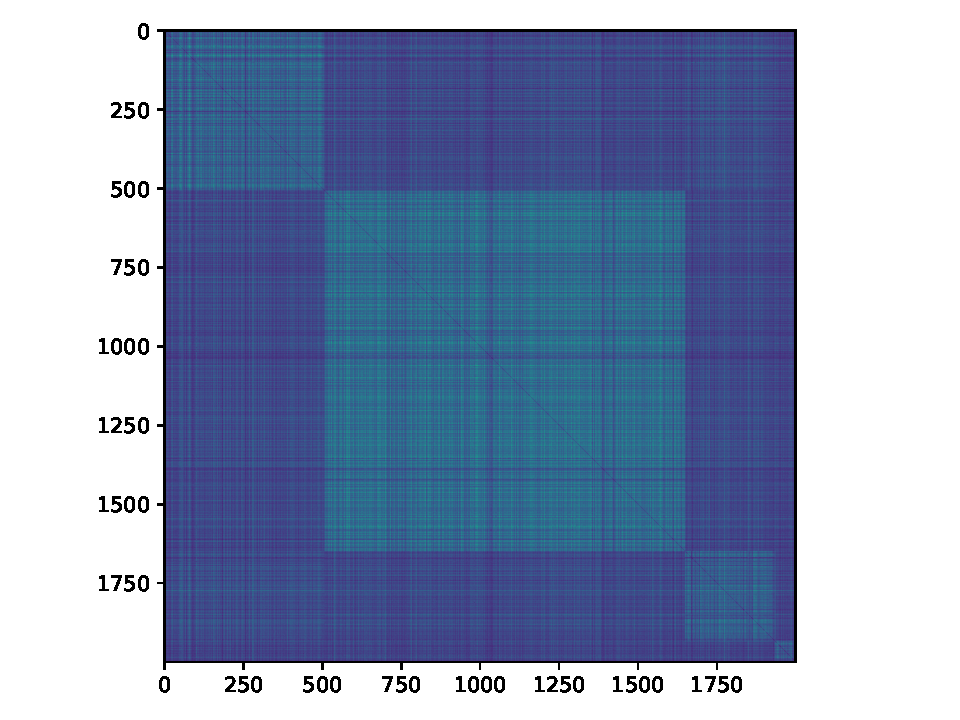
\includegraphics[width=7cm]{images/test_bad_true.pdf} }}%
    \qquad
    \subfloat[Predicted labels ordering]
    {{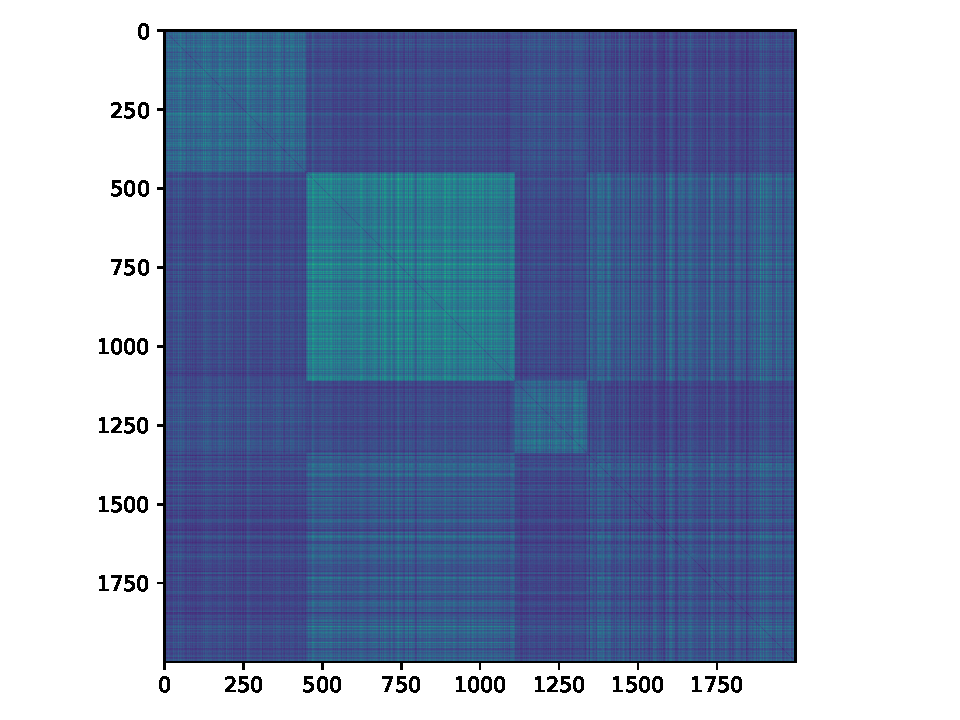
\includegraphics[width=7cm]{images/test_bad_pred.pdf} }}%
    \caption[Testing discovery matrices orderings]{Left: The sample of reads ordered according to their ground truth labels. Right: The ordering corresponding to the predicted labels.}%
    \label{fig:test_bad_discovery}
\end{figure}


As we can see from Tables \ref{tab:final_tests_all} and \ref{tab:final_test_classes}, our method algorithm works satisfactorily, almost always achieving a precision that would be suitable for practical purposes, sometimes for the slightly lower value of recall.

Somewhat disappointing is the accuracy of experiment $2$, in which the barcode $8$ was essentially omitted. Since we can observe lower precision of barcode $6$ in the same experiment, we hypothesize that the culprit is the cluster imbalancedness, since barcode $6$ appears with $\approx 20$ times higher frequency than barcode $8$ (see Fig. \ref{fig:barcodes_distribution}) in the dataset. Thus, a portion of the barcode $6$ gets classified as barcode $8$ during the discovery phase, which is then also reflected in the representatives selection and the errors are not averted by the final clustering of representatives.

This is confirmed in Fig. \ref{fig:test_bad_discovery}, which shows us the labels of the discovery sample score matrix in experiment $2$, ordered once for according to the ground truth labels and once according to the predicted labels. We can see that while in the ground truth labels ordering the classes are well defined albeit imbalanced, the prediction ordering divided the second cluster from the top (corresponding to barcode class $6$) into two of approximately the same size and labeled one of them as barcode $8$, which is represented in a severe minority in the sample (small square in the bottom right corner of the ground truth ordering).

Consequently to that, the contingency matrices of the set of representatives and the final test sample of $10,000$ squiggles look as follows (an example of an epoch from the test phase):
\bigskip

\begin{tabular}{ cc }% top level tables, with 2 columns
\label{tab:bad_test_contingencies}
Contingency table (representatives) & Contingency table for (test sample) \\  
\begin{tabular}{c|c|c|c|c}
& bc 5 & bc 6 & bc 7 & bc 8\\
\hline
bc 5 & 25 & 0 & 0 & 0\\
bc 6 & 0 & \textbf{19} & 0 & \textbf{6}\\
bc 7 & 0 & 0 & 25 & 0\\
bc 8 & 3 & 2 & 0 & 20
\end{tabular} &
\begin{tabular}{c|c|c|c|c}
& bc 5 & bc 6 & bc 7 & bc 8\\
\hline
bc 5 & 2196 & 5 & 5 & 9\\
bc 6 & 4 & \textbf{1753} & 13 & \textbf{1195}\\
bc 7 & 12 & 19 & 1296 & 8\\
bc 8 & 4 & 1 & 63 & 0 
\end{tabular}\\
\end{tabular}
\bigskip

Nevertheless, besides the pathological case of experiment $2$, we conclude that our algorithm performs satisfactorily.

\section{Time and Memory Complexity Analysis}
Let us now look into the asymptotic time and memory complexities of our approach. First, we examine the discovery phase. Similarly to classical DTW, a single LDTW computation takes $O(N \cdot M)$ time for squiggles of lengths $N,M$, so computing the all-pairs scores for a sample of size $n$ and the window size of $w$ is $w^2 \binom{n}{2}$. The time complexity of spectral clustering is $O(n^3)$ due to its eigenvalue decomposition step, which is costly in general \cite{shi2000normalized}. The representative selection is done in $O(kn^2)$ for $k$ being the number of clusters, since we need to iterate through the discovery matrix for each class. Putting that together, we have

\begin{multline}
    T_{\text{discovery}}(n, k, w) = T_{\text{score-matrix}}(n, w) +  T_{\text{spectral}}(n) + T_{\text{selection}}(n, k) =\\= \frac{w^2(n^2 - n)}{2} + O(n^3) + O(kn^2) \in O(n^3 + n^2w^2 + kn^2).
\end{multline}

Further on, if $m$ is the number of reads clustered in the clustering phase, the number of barcodes used is $k$ and the number of representatives selected from each barcode in the discovery phase is $r$, the time complexity of the clustering phase is then
\begin{equation}
    T_{\text{clustering}}(m, r, k, w) = mrkw^2 \in \Theta(mrk w^2).
\end{equation}

From the point of view of a particular experiment, $k, r, w$ are fixed constants. Considering that, we arrive with a cubic time complexity for the discovery phase, but only linear time for the clustering phase, which is feasible as it was our original goal. However, in practice $m$ can grow to the order of millions, so the constant factor is still important to us.

The discovery phase scales worse due to its cubic growth that comes from spectral clustering. In practice, the size of the initial sample should be motivated by the number of barcodes used in the experiment as we would like to have each class represented reasonably well.

We benefit greatly from the utilization of multithreading as both discovery and clustering phases are both easily parallelizable and with a $N_{\text{threads}}$ available threads we effectively get a corresponding speed-up factor. Hence, our approach works best on CPUs with large number of threads.

As far as memory complexity is concerned, our solution is very economic, requiring only to store a matrix of size $n^2$ in the discovery phase. The clustering phase then continues in a stream-like manner, keeping only the $r$ representatives out of each $k$ clusters and these numbers do not grow in time. The reads that are being processed can be read from a storage device. We can conclude that our solution is very efficient memory-wise and does not need an amount of memory beyond of what is the current standard in personal computers.

It is important to note that for our solution to work satisfactorily, we need to sample a sufficient amount of squiggles from every barcode class in our discovery phase, so the sample size needs to be scaled proportionally with the number of barcodes used. This is a toll for our unsupervised approach. Additionally, we also have to take into consideration the number of representatives we want to select from each class when setting the initial sample size. We did not explore the level of dependency of classification accuracy on the number of representatives used, but our hypothesis is that the robustness of our algorithm depends, at least to some extent, on the number of representatives used for each class.

As ONT barcode kits provide up to $96$ barcodes, the usability of all $96$ barcodes at once in a sequencing run can provide problematic, mainly for its difficulty in the discovery phase. However, many experimental settings employ only significantly smaller numbers of barcodes, oftentimes as few as $2$ or $3$, where our approach works reliably (see Tab. \ref{tab:final_tests_all}). It is also important to point out that putting more computation time into the discovery phase increases the chance of finding representatives of better quality and subsequently allows for a higher clustering accuracy.

Hence we have a trade-off between accuracy and CPU time consumption. This brief analysis should not be taken for a decision making guideline, but serve merely informatively for the experimenter, on which the final choice of the parameters if left.

\subsection{Time Measurements}
We briefly provide some measurements of several runs of our implementation. Our time measurements were performed on a Intel Xeon CPU E5-$2670$ $0$ @ $2.60$GHz, utilizing all of its $16$ cores.

Since computing the LDTW scores between all pairs of squiggles from a sample makes the bulk of the algorithm in terms of computational time, we will measure only those parts and neglect the rest. The results are summarized in table \ref{tab:time_measurements}.

\begin{table}[!ht]
\centering
\begin{tabular}{|c|cccccc|}
\hline
$N$ & 50  & 200  & 500  & 1000  & 2000  & 4000\\
\hline
\text{time (sec.)} & 0.97 & 12.8 & 77.4 & 307.8 & 1211.6 & 4742.9\\  \hline
\end{tabular}
\caption{Time measurements of computing all pairs of LDTW scores from a sample of size $N$. Each squiggle from the sample was $1000$ in length. The measurements are an average out of $5$ runs.}
\label{tab:time_measurements}
\end{table}

\section{Experiment: Inference of the Number of Clusters}
In the idea of an experiment where the barcodes are randomly generated in an isolated oil sphere, their structure as well as their count is unknown prior to the execution of the experiment. The number of generated barcodes is, however, potentially high. To the best of our knowledge, such experiment has not been performed yet due to nonexistence of demultiplexing tool able to infer the correct number of barcodes and cluster the squiggles without apriori knowing their structure. The motivation behind this idea is its vast applicability in cancer research, personalized medicine, etc.

As we would like to examine the suitability of our unsupervised barcode demultiplexing algorithm to this problem, the question we will address in this Section is the one of inferring the number of barcode classes by perceiving the pairwise LDTW scores of samples, taking into account that the number of barcodes can potentially be high.

Inferring the optimal number of clusters is a hard problem and no general solution that guarantees to work satisfactorily exists, apart from the model based clustering techniques, where it is sometimes a well-defined and efficiently solvable problem \cite{von2007tutorial}. However, several heuristics have been developed to tackle the general version of this task.

In spectral clustering, it is a well-known heuristic to estimate the optimal number of clusters $k$ as

\begin{equation}
    k = \arg \max_{i} |\lambda_{i+1} - \lambda_{i}|
\end{equation}

where $\lambda_1 \leq \lambda_2 \leq ... \leq \lambda_{m}$ are the eigenvalues of the Laplacian matrix sorted in non-decreasing order. This heuristic known as \textit{eigen-gap} (or \textit{spectral gap}) - the name refers to the largest gap in a sequence of sorted eigenvalues $\lambda_1, ..., \lambda_m$. However, for the heuristic to work as desired, the clusters need to be well pronounced in the data, without much noise or overlaps \cite{von2007tutorial}. The motivation for this heuristic follows from the perturbation theory \cite{von2007tutorial}. 

The smallest eigenvalue of a Laplacian is $0$, with its multiplicity equal to the number of connected components \cite{von2007tutorial}. Hence, to employ such heuristic, we should ensure the graph we are working with is connected, otherwise the optimal number of clusters equals the number of connected components. 

Another method that could be used for cluster number inference is the utilization of silhouette score as some form of a 'validation' of each choice of $k$ - since silhouette score measures how natural the clustering is given the data similarities, the $k$ yielding the highest silhouette score should be treated as the most natural number of clusters with regards to the data \cite{silhouette1987}. Others methods include information theory and other ad hoc measures \cite{von2007tutorial}.

\subsection{Experimental Results}
We experimented with eigen-gap and silhouette score methods of the cluster number inference. 
Naturally to our approach, we will try to estimate the number of clusters from a discovery matrix. We will test the heuristics using a sample of squiggles of size $4000$ sampled from the Deepbinner dataset of barcodes $1-8$ with a distribution summarized displayed Tab. \ref{tab:8bc_distribution}. From the LDTW score matrix of this sample we construct a $k$NN graph for $k=50$, which will be used as an input for the mentioned methods.

\begin{table}[!ht]
\centering
\begin{tabular}{|c|cccccccc|c|}
\hline
Barcode & 1   & 2   & 3   & 4   & 5   & 6    & 7   & 8 & Total \\
\hline
Count   & 274 & 824 & 452 & 261 & 553 & 1232 & 319 & 85 & 4000\\
\hline
\end{tabular}
\caption{The distribution of barcode classes sampled for the inference number of clusters.}
\label{tab:8bc_distribution}
\end{table}

As we can see from Fig. \ref{fig:clusters_estimation}, we have not been able to infer the exact number of clusters, although the estimated numbers of clusters are close lower bounds and so could potentially be useful in estimation of the correct number. These results may be improved by a more suitable method of graph construction. We leave further exploration of this problem for future studies.

\begin{figure}[!ht]
    \centering
    \subfloat[Eigen-gap heuristic]
    {{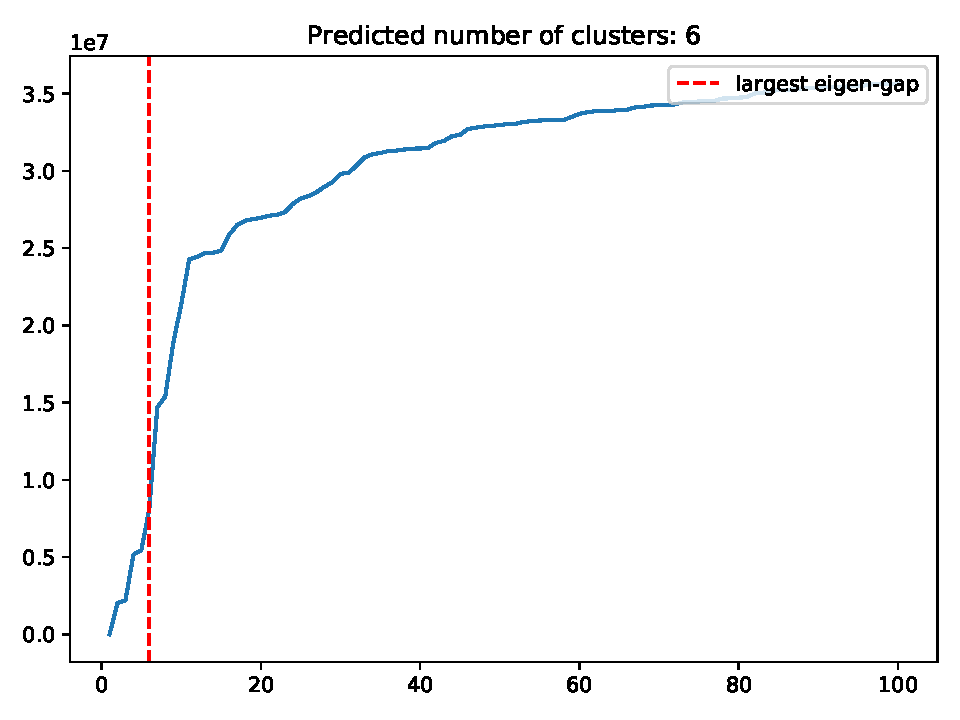
\includegraphics[width=7cm]{images/4000_8_eig.pdf} }}%
    \qquad
    \subfloat[Silhouette heuristic]
    {{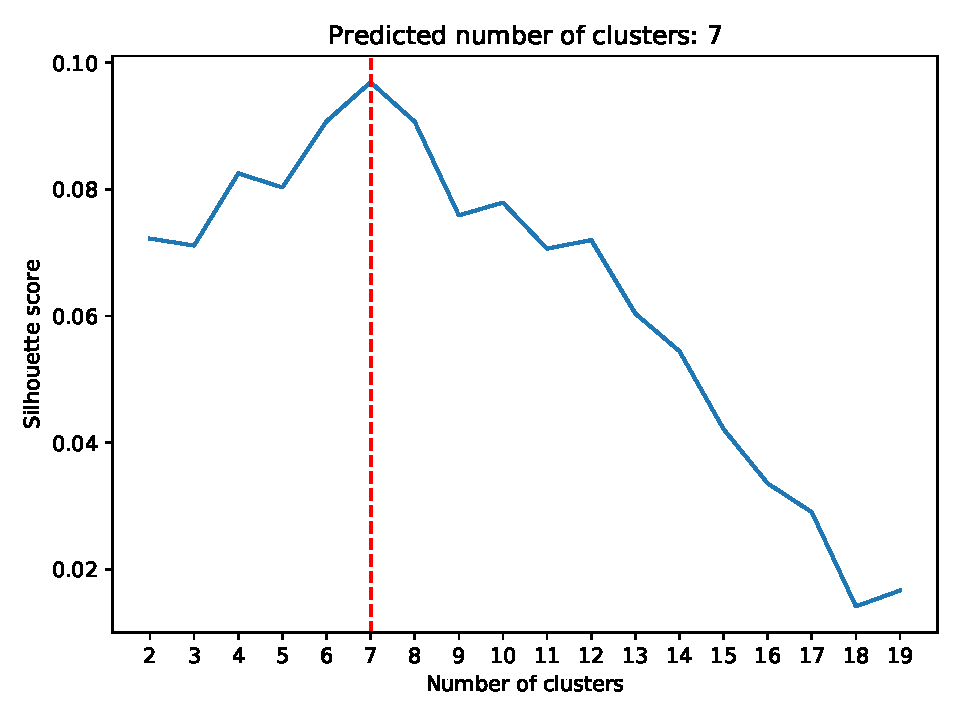
\includegraphics[width=7cm]{images/4000_8_silh.pdf} }}%
    \caption[Scoring scheme construction.]{Left: The plot of the sorted eigenvalues $\lambda_1, ..., \lambda_{100}$. Right: The results of the silhouette score heuristic. As we can see, even though the maximal \textbf{S} is attained at $7$, both of the values $6,8$ are almost as large.}%
    \label{fig:clusters_estimation}%
\end{figure}


\section{Experiment: Supervised Setting}
As we have assessed the performance of our unsupervised algorithm and compared it to Deepbinner, let us now consider its supervised alternative to make a comparison with equal conditions.

We sample a $500$ squiggles from each of the barcode classes $1-4$ of the Deepbinner dataset, compute the pairwise similarities and select $25$ representatives out of each class with the \textbf{means-ratio} method using \textbf{ground truth} labels (as opposed to using the predicted labels in the unsupervised setting). This part roughly corresponds to the training of the CNN that Deepbinner uses for classification.

Subsequently we sample a test sample of size $50,000$ squiggles that we classify using the \textbf{maxmean} method together with the $\tau = 0.9$ for the ambiguous labels detection criterium. 

The results are displayed in Tab. \ref{tab:supervised_overall} and \ref{tab:supervised_classes}. We can see that the performance of our model is comparable to that of Deepbinner's, achieving only a slightly less satisfactory results. However, we note that our results are not directly comparable to Deepbinner's due to different experimental settings. It is possible that with more time invested into the tuning of the parameters of our model, we might be able to surpass the performance of Deepbinner, nonetheless we showed that our approach is suitable for use in supervised setting as well. In contrast with Deepbinner's CNN model, the one we use is much smaller in size, takes far shorter time to train and perhaps most importantly - is interpretable, which is a property that neural network based models inherently lack.

\begin{table}[!ht]
\centering
\begin{tabular}{|l|ccccc|}
\hline
& ARI &  F$1$ & Precision (\%) & Recall (\%) & Binned reads\\
\hline
\text{our approach} & 0.96 & 0.95 & 98.39 & 91.35 & 92.84\\
\text{Deepbinner} & - & - & 98.41 & 93.33 & 94.84\\
\hline
\end{tabular}
\caption{The overall performance of the supervised approach on barcodes $1-4$ compared to the accuracy of Deepbinner \cite{Deepbinner}.}
\label{tab:supervised_overall}
\end{table}

\begin{table}[!ht]
\centering
\begin{tabular}{|l|cccc|}
\hline
& barcode 1 & barcode 2 & barcode 3 & barcode 4\\
\hline
Precision (\%) & 96.55 & 98.93 & 98.42 & 98.53\\
Recall (\%) & 86.39 & 93.25 & 91.12 & 91.00\\
\hline
\end{tabular}
\caption{The performance of the supervised approach across individual barcodes.}
\label{tab:supervised_classes}
\end{table}
